\documentclass{article}
\usepackage[margin=2.5cm]{geometry} % Adjust the margin value as desired

\usepackage{amsmath}
\usepackage{amsfonts}
\usepackage{float}
\usepackage{cite}

\usepackage{tikz}
\usetikzlibrary {arrows.meta} 
\usepackage{xcolor}

\newcommand{\C}{\mathcal{C}}
\newcommand{\N}{\mathbb{N}}

\definecolor{navyblue}{rgb}{0.0, 0.0, 0.5}
\definecolor{forestgreen}{rgb}{0.13, 0.55, 0.13}
\definecolor{darkred}{rgb}{0.59, 0.0, 0.09}
\definecolor{darkblue}{rgb}{0.0, 0.18, 0.39}

\title{Models of Computation - Colored Graphs}
\author{Nils Cremer}
\date{\today}

\begin{document}

\maketitle

\section{Motivation}

In this report, I will present a model of computation that I call Colored Graphs.
The motivation behind it is to a more parallel and asynchronous model of computation than let's say the very sequential Turing Machine.
But also to not be restricted by a fixed topology like is the case in cellular automata.
To be able to encode "closeness" of things that belong to each other, e.g. a function and its argument, a graph is natural representation of these kinds of relationships.
Secondly, I wanted the model to be as minimal as I could make it.
It stated out with quite general graph rewriting where large parts of the graph could be added and edges added and removed.
After some simplifications, I ended up with the model that is only comprised of two simple kinds and very local rules.

\section{Colored Graphs}

In this section, I will explain my model of computation which I call Colored Graphs.
It consists of a simple (undirected, no multi-edges, no loops) graph $G = (V, E)$,
together with an edge coloring $c : E \to \C$ that assigns each edge a color from a finite set of Colors $\C$.
You can find an example of a graph below.

\begin{figure}[H]
    \label{fig:graph1}
    \centering
    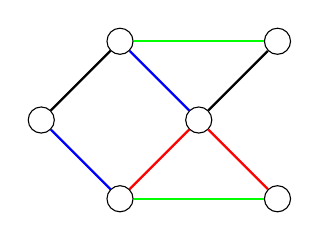
\begin{tikzpicture}
        \node[circle,draw] (A) at (1,-1) {};
        \node[circle,draw] (B) at (2,0) {};
        \node[circle,draw] (C) at (1,1) {};
        \node[circle,draw] (D) at (3,1) {};
        \node[circle,draw] (E) at (3,-1) {};
        \node[circle,draw] (F) at (0,0) {};
        
        \draw[red, thick] (A) -- (B);
        \draw[blue, thick] (B) -- (C);
        \draw[green, thick] (C) -- (D);
        \draw[black, thick] (B) -- (D);
        \draw[green, thick] (E) -- (A);
        \draw[blue, thick] (F) -- (A);
        \draw[black, thick] (F) -- (C);
        \draw[red, thick] (B) -- (E);
    \end{tikzpicture}
    \caption{Example of a Colored Graph}
\end{figure}


The model computes by applying rules to the vertices of a graph which I will first describe informally.
To determine whether a rule can be applied to a vertex of the graph, we look at the colors of incident edges to that vertex.
Concretely, an example rule might apply when a node is incident to 2 red edges and 1 black edge.
When a rule is being applied to a vertex, it changes the graph.
This, however, can not happen in an arbitrary way, but only in two simple ways.
First, the rule can delete the vertex and "rewire" the adjacent vertices, or secondly it can split the vertex in two independent nodes and connected the two vertices to the adjacent vertices of the original vertex.
Next I will describe the rules more formally.

\paragraph*{Delete Rule} A Delete Rule has a condition $b : \C \to \N$.
We say this rule can be applied to a vertex $v$ if the vertex has exactly $b(c)$ incident edges of color $c$ for all $c \in \C$.
If a Delete Rule is applied, the vertex $v$ is deleted and the adjacent vertices rewired.
Since the rule does not distinguish between different neighboring vertices nor different edges of the same color, the rewiring will be of the form "connect the vertices of the blue edges to the vertices of the red edges with a new yellow edge".
Or more formally we have a mapping $d: \C \times \C \rightharpoonup C$, that maps some pairs of colors to a new color.
Note that this in particular also allows a pair of the same color to be mapped to a new color.
This behaves basically in the same way as two different colors, by connecting all vertices connected by this color to each other.
However, no loops will be created, so vertices are not connected to themselves in that case.
In case the Delete Rule connects two vertices that are already connected, the new edge "overwrites" the old edge.

Instead of defining rules completely formally, I will mostly show them visually in the following way where the node the rule is applied to is marked in black.

\begin{center}
    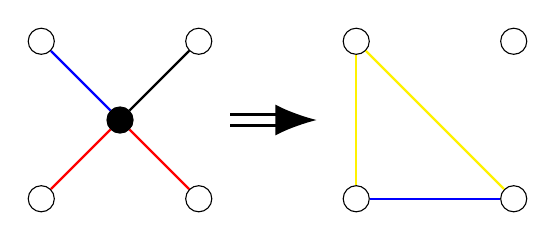
\begin{tikzpicture}
    \begin{scope}[xshift=-2cm]
        \node[circle,draw] (A) at (1,-1) {};
        \node[circle,draw,fill] (B) at (2,0) {};
        \node[circle,draw] (C) at (1,1) {};
        \node[circle,draw] (D) at (3,1) {};
        \node[circle,draw] (E) at (3,-1) {};
        
        \draw[red, thick] (A) -- (B);
        \draw[blue, thick] (B) -- (C);
        \draw[black, thick] (B) -- (D);
        \draw[red, thick] (B) -- (E);
    \end{scope}

    \draw [line width=1pt, double distance=3pt, arrows = {-Latex[length=0pt 3 0]}] (1.4,0) -- (2.5,0);
    
    \begin{scope}[xshift=2cm]
        \node[circle,draw] (A2) at (1,-1) {};
        \node[circle,draw] (C2) at (1,1) {};
        \node[circle,draw] (D2) at (3,1) {};
        \node[circle,draw] (E2) at (3,-1) {};
        
        \draw[blue, thick] (A2) -- (E2);
        \draw[yellow, thick] (A2) -- (C2);
        \draw[yellow, thick] (E2) -- (C2);
    \end{scope}
    \end{tikzpicture}
\end{center}

This represents a Delete Rule that can be applied to a node that had 2 incident red edges, one blue edge and a black edge.
After deletion of the node, it rewires the blue and red vertices with a yellow edge and the red vertices with itself with blue edges.
Notice that I will sometimes call the neighboring vertices "blue vertices" even though the vertices have no color themselves.
This is just shorthand for the vertices that are connected by a blue edge.
The rewiring of the rule above can also be formally describes as the mapping of the pairs of colors $(\text{red}, \text{blue}) \mapsto \text{yellow}$ and $(\text{red}, \text{red}) \mapsto \text{blue}$.

If we apply this rule to the middle vertex of the example graph in Figure \ref{fig:graph1}, we get the following graph.

\begin{figure}[H]
    \label{fig:graph2}
    \centering
    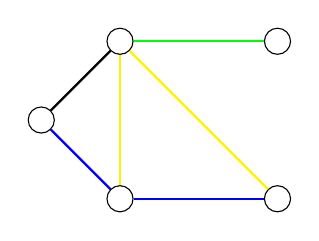
\begin{tikzpicture}
        \node[circle,draw] (A) at (1,-1) {};
        \node[circle,draw] (C) at (1,1) {};
        \node[circle,draw] (D) at (3,1) {};
        \node[circle,draw] (E) at (3,-1) {};
        \node[circle,draw] (F) at (0,0) {};
        
        \draw[green, thick] (C) -- (D);
        \draw[blue, thick] (E) -- (A);
        \draw[blue, thick] (F) -- (A);
        \draw[black, thick] (F) -- (C);
        \draw[yellow, thick] (A) -- (C);
        \draw[yellow, thick] (E) -- (C);
    \end{tikzpicture}
    \caption{Graph after applying the example Delete Rule}
\end{figure}

\paragraph*{Split Rule} A Split Rule has the same kind of condition $b : \C \to \N$ as a Delete Rule.
So again, we count the number of incident edges of each color to see if it matches the condition of the rule.
In contract to a Delete Rule, a Split Rule does not delete the vertex but splits it into two vertices.
The rule then determines which neighboring nodes the two new vertices are connected to.
Again, we don't distinguish vertices that are connected with the same color.
The new connections of the first node can we described by a mapping $s_1 : \C \rightharpoonup \C$ and the new connections of the second node by $s_2 : \C \rightharpoonup \C$.
These mapping describe the colors of the edges with which the two new vertices should be connected to some of the neighboring vertices.

An example Split Rule would be

\begin{center}
    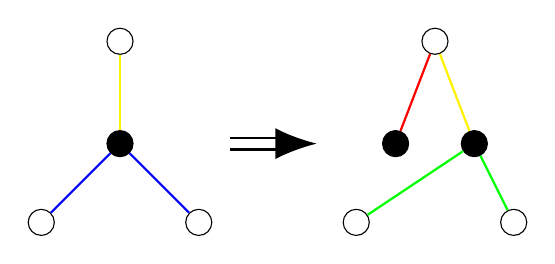
\begin{tikzpicture}
    \begin{scope}[xshift=-2cm]
        \node[circle,draw,fill] (B) at (2,0) {};

        \node[circle,draw] (A) at (1,-1) {};
        \node[circle,draw] (C) at (2,1.3) {};
        \node[circle,draw] (E) at (3,-1) {};
        
        \draw[blue, thick] (B) -- (A);
        \draw[yellow, thick] (B) -- (C);
        \draw[blue, thick] (B) -- (E);
    \end{scope}

    \draw [line width=1pt, double distance=3pt,
             arrows = {-Latex[length=0pt 3 0]}] (1.4,0) -- (2.5,0);
    
    \begin{scope}[xshift=2cm]
        \node[circle,draw,fill] (B2) at (2.5,0) {};
        \node[circle,draw,fill] (D2) at (1.5,0) {};
        
        \node[circle,draw] (A2) at (1,-1) {};
        \node[circle,draw] (C2) at (2,1.3) {};
        \node[circle,draw] (E2) at (3,-1) {};
        
        \draw[yellow, thick] (B2) -- (C2);
        \draw[green, thick] (B2) -- (A2);
        \draw[green, thick] (B2) -- (E2);
        \draw[red, thick] (D2) -- (C2);
    \end{scope}
    
    \end{tikzpicture}
\end{center}

It represents a Split Rule that can be applied to a node that had 2 incident blue edges and one yellow edge.
The two new nodes with their new edges can be described by the mapping $s_1$ that maps yellow to red and $s_2$ which maps blue to green and yellow to yellow.

Applying this rule to the bottom left node in the graph in Figure \ref{fig:graph2}, we get the following graph.

\begin{figure}[H]
    \label{fig:graph3}
    \centering
    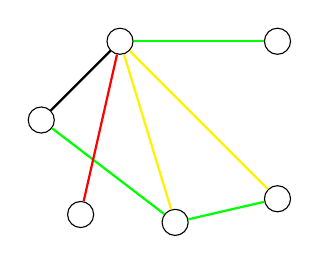
\begin{tikzpicture}
        \node[circle,draw] (A) at (1.7,-1.3) {};
        \node[circle,draw] (C) at (1,1) {};
        \node[circle,draw] (D) at (3,1) {};
        \node[circle,draw] (E) at (3,-1) {};
        \node[circle,draw] (F) at (0,0) {};
        \node[circle,draw] (G) at (0.5,-1.2) {};
        
        \draw[green, thick] (C) -- (D);
        \draw[green, thick] (E) -- (A);
        \draw[green, thick] (F) -- (A);
        \draw[black, thick] (F) -- (C);
        \draw[yellow, thick] (A) -- (C);
        \draw[yellow, thick] (E) -- (C);
        \draw[red, thick] (G) -- (C);
    \end{tikzpicture}
    \caption{Graph after applying the example Split Rule}
\end{figure}

\paragraph*{Computation}
A program in the Colored Graph model is a finite set of Delete and Split Rule.
The input to the model is an initial colored graph.
In each step of the computation an arbitrary rule is applied to a vertex that satisfies the condition of the rule.
This is repeated until no rule can be applied anymore.
Notice that this model is not necessarily confluent meaning that there might be different reductions that lead to different end results.
It is the task of the programmer to design rules and a suitable encoding of the problem input such that the computation always leads to the desired result no matter the order of rule applications.

I also implemented a simulator in Python which you can find in this GitHub repository \\
(https://github.com/nilscrm/colored-networks).
It also contains the examples that now follow.

\section{Example Computations}

To get feel for the model, let's look at some example computations.

\paragraph*{Addition}
Let's try to implement addition in the Colored Graph model.
We represent a number $n$ by a chain of $n+1$ nodes connected to each other with blue edges.
The reason that we use $n+1$ and not $n$ to be able to represent 0 with a single node.
Then to add two number, we will connect the two chains together with a red edge to a long chain.
So the input to our program to add 3 and 5 will be the following graph.

\begin{center}
    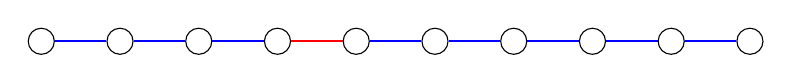
\begin{tikzpicture}
        \node[circle,draw] (A) at (1,0) {};
        \node[circle,draw] (B) at (2,0) {};
        \node[circle,draw] (C) at (3,0) {};
        \node[circle,draw] (D) at (4,0) {};

        \node[circle,draw] (E) at (5,0) {};
        \node[circle,draw] (F) at (6,0) {};
        \node[circle,draw] (G) at (7,0) {};
        \node[circle,draw] (H) at (8,0) {};
        \node[circle,draw] (I) at (9,0) {};
        \node[circle,draw] (J) at (10,0) {};
        
        \draw[blue, thick] (A) -- (B);
        \draw[blue, thick] (B) -- (C);
        \draw[blue, thick] (C) -- (D);
        \draw[red, thick] (D) -- (E);
        \draw[blue, thick] (E) -- (F);
        \draw[blue, thick] (F) -- (G);
        \draw[blue, thick] (G) -- (H);
        \draw[blue, thick] (H) -- (I);
        \draw[blue, thick] (I) -- (J);
    \end{tikzpicture}
\end{center}

To add these two numbers we simply need the following rule.

\begin{center}
    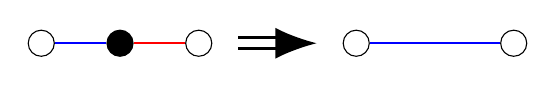
\begin{tikzpicture}
    \begin{scope}[xshift=-2cm]
        \node[circle,draw] (A) at (-1, 0) {};
        \node[circle,draw,fill] (B) at (0,0) {};
        \node[circle,draw] (C) at (1,0) {};
        
        \draw[blue, thick] (A) -- (B);
        \draw[red, thick] (B) -- (C);
    \end{scope}

    \draw [line width=1pt, double distance=3pt, arrows = {-Latex[length=0pt 3 0]}] (-0.5,0) -- (0.5,0);
    
    \begin{scope}[xshift=2cm]
        \node[circle,draw] (A) at (-1, 0) {};
        \node[circle,draw] (C) at (1,0) {};
        
        \draw[blue, thick] (A) -- (C);
    \end{scope}
    \end{tikzpicture}
\end{center}

This rule can be applied to either of the nodes connected to the red edge and in one step will produce the correct restult.

\begin{center}
    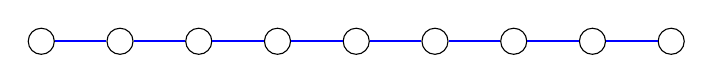
\begin{tikzpicture}
        \node[circle,draw] (A) at (1,0) {};
        \node[circle,draw] (B) at (2,0) {};
        \node[circle,draw] (C) at (3,0) {};
        \node[circle,draw] (D) at (4,0) {};

        \node[circle,draw] (E) at (5,0) {};
        \node[circle,draw] (F) at (6,0) {};
        \node[circle,draw] (G) at (7,0) {};
        \node[circle,draw] (H) at (8,0) {};
        \node[circle,draw] (I) at (9,0) {};
        
        \draw[blue, thick] (A) -- (B);
        \draw[blue, thick] (B) -- (C);
        \draw[blue, thick] (C) -- (D);
        \draw[blue, thick] (D) -- (E);
        \draw[blue, thick] (E) -- (F);
        \draw[blue, thick] (F) -- (G);
        \draw[blue, thick] (G) -- (H);
        \draw[blue, thick] (H) -- (I);
    \end{tikzpicture}
\end{center}

To deal with the special case of $0 + 0$, for which this rule does not work we will add the following Delete Rule that just removes a node connected to exactly one red edge and has an empty rewiring.

\begin{center}
    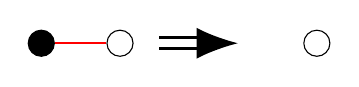
\begin{tikzpicture}
    \begin{scope}[xshift=-2cm]
        \node[circle,draw,fill] (B) at (0,0) {};
        \node[circle,draw] (C) at (1,0) {};
        
        \draw[red, thick] (B) -- (C);
    \end{scope}

    \draw [line width=1pt, double distance=3pt, arrows = {-Latex[length=0pt 3 0]}] (-0.5,0) -- (0.5,0);
    
    \begin{scope}[xshift=2cm]
        \node[circle,draw] (C) at (-0.5,0) {};
    \end{scope}
    \end{tikzpicture}
\end{center}

That was pretty easy so let's turn to some more complex examples.

\paragraph*{Shortest distance}

As one could imagine representing graph problems in this model is quite natural.
However, maybe not as natural as one might think.
The main problem is that most graph problems can have graphs with nodes of arbitrary degree.
Rules in our model can only apply to nodes of a fixed degree though and since we only have finitely many rules, nodes with a very high degree become a problem as no rule could be applied.
I will show a technique to overcome this challenge.
The problem we want to solve is to determine the length of the shortest path between two given nodes $u$ and $v$ in a simple connected graph.
We will make our lives a bit easier by assuming $u \ne v$.

To visualize the process I will use this example graph.

\begin{center}
    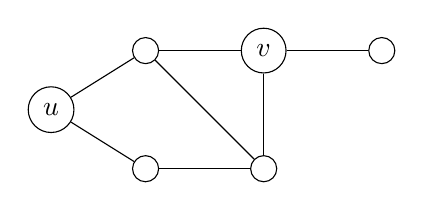
\begin{tikzpicture}
        \node[circle,draw] (v0) at (-0.2,0.75) {$u$};
        \node[circle,draw] (v1) at (1,1.5) {};
        \node[circle,draw] (v2) at (1,0) {};
        \node[circle,draw] (v3) at (2.5,1.5) {$v$};
        \node[circle,draw] (v4) at (2.5,0) {};
        \node[circle,draw] (v5) at (4,1.5) {};

        \draw (v0) -- (v1);
        \draw (v0) -- (v2);
        \draw (v1) -- (v3);
        \draw (v1) -- (v4);
        \draw (v2) -- (v4);
        \draw (v3) -- (v4);
        \draw (v3) -- (v5);
    \end{tikzpicture}
\end{center}

I will show step for step how we will encode this input graph as a Colored Graph.
First, to overcome the problem mentioned before of arbitrary degree, we will encode every vertex of the input as ring of nodes.
Then each node in a given vertex ring is only incident to one edge of the original graph.
The ring nodes are connected with black edges while the edges between vertices are green.

\begin{center}
    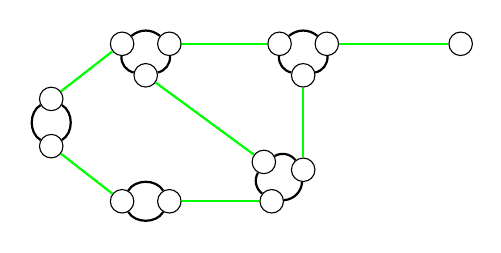
\begin{tikzpicture}
        \node[circle,draw,inner sep=3pt] (v00) at (-0.2,0.7) {};
        \node[circle,draw,inner sep=3pt] (v01) at (-0.2,1.3) {};
        \node[circle,draw,inner sep=3pt] (v10) at (0.7,2) {};
        \node[circle,draw,inner sep=3pt] (v11) at (1,1.6) {};
        \node[circle,draw,inner sep=3pt] (v12) at (1.3,2) {};
        \node[circle,draw,inner sep=3pt] (v20) at (0.7,0) {};
        \node[circle,draw,inner sep=3pt] (v21) at (1.3,0) {};
        \node[circle,draw,inner sep=3pt] (v30) at (2.7,2) {};
        \node[circle,draw,inner sep=3pt] (v31) at (3,1.6) {};
        \node[circle,draw,inner sep=3pt] (v32) at (3.3,2) {};
        \node[circle,draw,inner sep=3pt] (v40) at (2.6,0) {};
        \node[circle,draw,inner sep=3pt] (v41) at (2.5,0.5) {};
        \node[circle,draw,inner sep=3pt] (v42) at (3,0.4) {};
        \node[circle,draw,inner sep=3pt] (v5) at (5,2) {};

        \draw[thick,bend right=60] (v00) to (v01);
        \draw[thick,bend left=60] (v00) to (v01);
        \draw[thick,bend left=40] (v10) to (v12);
        \draw[thick,bend left=40] (v12) to (v11);
        \draw[thick,bend left=40] (v11) to (v10);
        \draw[thick,bend right=60] (v20) to (v21);
        \draw[thick,bend left=60] (v20) to (v21);
        \draw[thick,bend left=40] (v30) to (v32);
        \draw[thick,bend left=40] (v32) to (v31);
        \draw[thick,bend left=40] (v31) to (v30);
        \draw[thick,bend left=40] (v40) to (v41);
        \draw[thick,bend left=40] (v41) to (v42);
        \draw[thick,bend left=40] (v42) to (v40);

        \draw[thick,green] (v00) -- (v20);
        \draw[thick,green] (v01) -- (v10);
        \draw[thick,green] (v12) -- (v30);
        \draw[thick,green] (v11) -- (v41);
        \draw[thick,green] (v21) -- (v40);
        \draw[thick,green] (v31) -- (v42);
        \draw[thick,green] (v32) -- (v5);
    \end{tikzpicture}
\end{center}

Because we will perform a form of BFS on the graph we need some sense of direntionality in the edges.
Not in the sense that we can only go along the in one direction, but in the sense that we remember from which side an update originated.
To to this we will insert a node inbetween each edge.
This also result in no more multi-edges.
We will also extend any node of degree one (so for our example graph the node on the right) with an additional node so that it too becomes a proper ring.
That way the rules will get slightly simpler.

\begin{center}
    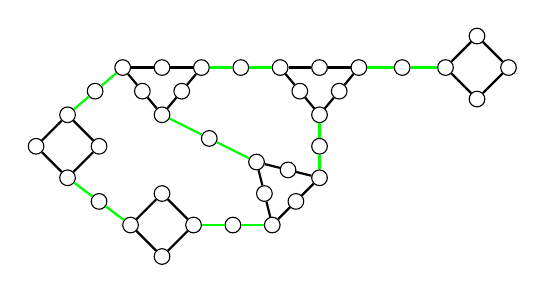
\begin{tikzpicture}
        \node[circle,draw,inner sep=2pt] (v00) at (-0.2,0.6) {};
        \node[circle,draw,inner sep=2pt] (v01) at (-0.2,1.4) {};
        \node[circle,draw,inner sep=2pt] (v02) at (-0.6,1) {};
        \node[circle,draw,inner sep=2pt] (v03) at (0.2,1) {};

        \node[circle,draw,inner sep=2pt] (c01) at (0.15,1.7) {};

        \node[circle,draw,inner sep=2pt] (v10) at (0.5,2) {};
        \node[circle,draw,inner sep=2pt] (v11) at (1,1.4) {};
        \node[circle,draw,inner sep=2pt] (v12) at (1.5,2) {};
        \node[circle,draw,inner sep=2pt] (v13) at (0.75,1.7) {};
        \node[circle,draw,inner sep=2pt] (v14) at (1.25,1.7) {};
        \node[circle,draw,inner sep=2pt] (v15) at (1,2) {};

        \node[circle,draw,inner sep=2pt] (c02) at (0.2,0.3) {};

        \node[circle,draw,inner sep=2pt] (v20) at (0.6,0) {};
        \node[circle,draw,inner sep=2pt] (v21) at (1.4,0) {};
        \node[circle,draw,inner sep=2pt] (v22) at (1,-0.4) {};
        \node[circle,draw,inner sep=2pt] (v23) at (1,0.4) {};

        \node[circle,draw,inner sep=2pt] (c13) at (2,2) {};

        \node[circle,draw,inner sep=2pt] (v30) at (2.5,2) {};
        \node[circle,draw,inner sep=2pt] (v31) at (3,1.4) {};
        \node[circle,draw,inner sep=2pt] (v32) at (3.5,2) {};
        \node[circle,draw,inner sep=2pt] (v33) at (2.75,1.7) {};
        \node[circle,draw,inner sep=2pt] (v34) at (3.25,1.7) {};
        \node[circle,draw,inner sep=2pt] (v35) at (3,2) {};

        \node[circle,draw,inner sep=2pt] (c14) at (1.6,1.1) {};
        \node[circle,draw,inner sep=2pt] (c24) at (1.9,0) {};
        \node[circle,draw,inner sep=2pt] (c34) at (3,1) {};
    
        \node[circle,draw,inner sep=2pt] (v40) at (2.4,0) {};
        \node[circle,draw,inner sep=2pt] (v41) at (2.2,0.8) {};
        \node[circle,draw,inner sep=2pt] (v42) at (3,0.6) {};
        \node[circle,draw,inner sep=2pt] (v43) at (2.3,0.4) {};
        \node[circle,draw,inner sep=2pt] (v44) at (2.6,0.7) {};
        \node[circle,draw,inner sep=2pt] (v45) at (2.7,0.3) {};

        \node[circle,draw,inner sep=2pt] (c35) at (4.05,2) {};

        \node[circle,draw,inner sep=2pt] (v50) at (5,1.6) {};
        \node[circle,draw,inner sep=2pt] (v51) at (5,2.4) {};
        \node[circle,draw,inner sep=2pt] (v52) at (4.6,2) {};
        \node[circle,draw,inner sep=2pt] (v53) at (5.4,2) {};

        \draw[thick] (v00) to (v02);
        \draw[thick] (v02) to (v01);
        \draw[thick] (v01) to (v03);
        \draw[thick] (v03) to (v00);

        \draw[thick] (v10) to (v13);
        \draw[thick] (v13) to (v11);
        \draw[thick] (v11) to (v14);
        \draw[thick] (v14) to (v12);
        \draw[thick] (v12) to (v15);
        \draw[thick] (v15) to (v10);

        \draw[thick] (v20) to (v22);
        \draw[thick] (v22) to (v21);
        \draw[thick] (v21) to (v23);
        \draw[thick] (v23) to (v20);

        \draw[thick] (v30) to (v33);
        \draw[thick] (v33) to (v31);
        \draw[thick] (v31) to (v34);
        \draw[thick] (v34) to (v32);
        \draw[thick] (v32) to (v35);
        \draw[thick] (v35) to (v30);

        \draw[thick] (v40) to (v43);
        \draw[thick] (v43) to (v41);
        \draw[thick] (v41) to (v44);
        \draw[thick] (v44) to (v42);
        \draw[thick] (v42) to (v45);
        \draw[thick] (v45) to (v40);

        \draw[thick] (v50) to (v52);
        \draw[thick] (v52) to (v51);
        \draw[thick] (v51) to (v53);
        \draw[thick] (v53) to (v50);

        \draw[thick,green] (v00) -- (c02);
        \draw[thick,green] (c02) -- (v20);

        \draw[thick,green] (v01) -- (c01);
        \draw[thick,green] (c01) -- (v10);

        \draw[thick,green] (v12) -- (c13);
        \draw[thick,green] (c13) -- (v30);

        \draw[thick,green] (v11) -- (c14);
        \draw[thick,green] (c14) -- (v41);

        \draw[thick,green] (v21) -- (c24);
        \draw[thick,green] (c24) -- (v40);

        \draw[thick,green] (v31) -- (c34);
        \draw[thick,green] (c34) -- (v42);

        \draw[thick,green] (v32) -- (c35);
        \draw[thick,green] (c35) -- (v52);
    \end{tikzpicture}
\end{center}

As a last step we will mark the start end end vertex.
To do this we insert a node into each ring and connect the start vertex to a dummy vertex with red and the goal vertex with blue.

\begin{center}
    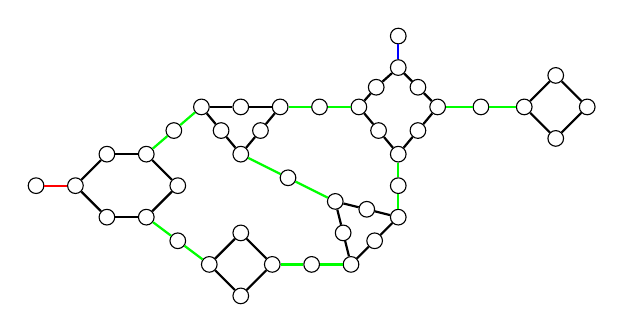
\begin{tikzpicture}
        \node[circle,draw,inner sep=2pt] (v00) at (-0.2,0.6) {};
        \node[circle,draw,inner sep=2pt] (v01) at (-0.2,1.4) {};
        \node[circle,draw,inner sep=2pt] (v02) at (-0.7,1.4) {};
        \node[circle,draw,inner sep=2pt] (v03) at (0.2,1) {};
        \node[circle,draw,inner sep=2pt] (v04) at (-0.7,0.6) {};
        \node[circle,draw,inner sep=2pt] (v05) at (-1.1,1) {};

        \node[circle,draw,inner sep=2pt] (s) at (-1.6,1) {};

        \node[circle,draw,inner sep=2pt] (c01) at (0.15,1.7) {};

        \node[circle,draw,inner sep=2pt] (v10) at (0.5,2) {};
        \node[circle,draw,inner sep=2pt] (v11) at (1,1.4) {};
        \node[circle,draw,inner sep=2pt] (v12) at (1.5,2) {};
        \node[circle,draw,inner sep=2pt] (v13) at (0.75,1.7) {};
        \node[circle,draw,inner sep=2pt] (v14) at (1.25,1.7) {};
        \node[circle,draw,inner sep=2pt] (v15) at (1,2) {};

        \node[circle,draw,inner sep=2pt] (c02) at (0.2,0.3) {};

        \node[circle,draw,inner sep=2pt] (v20) at (0.6,0) {};
        \node[circle,draw,inner sep=2pt] (v21) at (1.4,0) {};
        \node[circle,draw,inner sep=2pt] (v22) at (1,-0.4) {};
        \node[circle,draw,inner sep=2pt] (v23) at (1,0.4) {};

        \node[circle,draw,inner sep=2pt] (c13) at (2,2) {};

        \node[circle,draw,inner sep=2pt] (v30) at (2.5,2) {};
        \node[circle,draw,inner sep=2pt] (v31) at (3,1.4) {};
        \node[circle,draw,inner sep=2pt] (v32) at (3.5,2) {};
        \node[circle,draw,inner sep=2pt] (v33) at (2.75,1.7) {};
        \node[circle,draw,inner sep=2pt] (v34) at (3.25,1.7) {};
        \node[circle,draw,inner sep=2pt] (v35) at (3.25,2.25) {};
        \node[circle,draw,inner sep=2pt] (v36) at (3,2.5) {};
        \node[circle,draw,inner sep=2pt] (v37) at (2.72,2.25) {};

        \node[circle,draw,inner sep=2pt] (g) at (3,2.9) {};

        \node[circle,draw,inner sep=2pt] (c14) at (1.6,1.1) {};
        \node[circle,draw,inner sep=2pt] (c24) at (1.9,0) {};
        \node[circle,draw,inner sep=2pt] (c34) at (3,1) {};
    
        \node[circle,draw,inner sep=2pt] (v40) at (2.4,0) {};
        \node[circle,draw,inner sep=2pt] (v41) at (2.2,0.8) {};
        \node[circle,draw,inner sep=2pt] (v42) at (3,0.6) {};
        \node[circle,draw,inner sep=2pt] (v43) at (2.3,0.4) {};
        \node[circle,draw,inner sep=2pt] (v44) at (2.6,0.7) {};
        \node[circle,draw,inner sep=2pt] (v45) at (2.7,0.3) {};
        
        \node[circle,draw,inner sep=2pt] (c35) at (4.05,2) {};

        \node[circle,draw,inner sep=2pt] (v50) at (5,1.6) {};
        \node[circle,draw,inner sep=2pt] (v51) at (5,2.4) {};
        \node[circle,draw,inner sep=2pt] (v52) at (4.6,2) {};
        \node[circle,draw,inner sep=2pt] (v53) at (5.4,2) {};

        \draw[thick,red] (s) to (v05);

        \draw[thick] (v00) to (v04);
        \draw[thick] (v05) to (v04);
        \draw[thick] (v02) to (v05);
        \draw[thick] (v02) to (v01);
        \draw[thick] (v01) to (v03);
        \draw[thick] (v03) to (v00);

        \draw[thick] (v10) to (v13);
        \draw[thick] (v13) to (v11);
        \draw[thick] (v11) to (v14);
        \draw[thick] (v14) to (v12);
        \draw[thick] (v12) to (v15);
        \draw[thick] (v15) to (v10);

        \draw[thick] (v20) to (v22);
        \draw[thick] (v22) to (v21);
        \draw[thick] (v21) to (v23);
        \draw[thick] (v23) to (v20);

        \draw[thick] (v30) to (v33);
        \draw[thick] (v33) to (v31);
        \draw[thick] (v31) to (v34);
        \draw[thick] (v34) to (v32);
        \draw[thick] (v32) to (v35);
        \draw[thick] (v35) to (v36);
        \draw[thick] (v36) to (v37);
        \draw[thick] (v37) to (v30);

        \draw[thick, blue] (v36) to (g);

        \draw[thick] (v40) to (v43);
        \draw[thick] (v43) to (v41);
        \draw[thick] (v41) to (v44);
        \draw[thick] (v44) to (v42);
        \draw[thick] (v42) to (v45);
        \draw[thick] (v45) to (v40);

        \draw[thick] (v50) to (v52);
        \draw[thick] (v52) to (v51);
        \draw[thick] (v51) to (v53);
        \draw[thick] (v53) to (v50);

        \draw[thick,green] (v00) -- (c02);
        \draw[thick,green] (c02) -- (v20);

        \draw[thick,green] (v01) -- (c01);
        \draw[thick,green] (c01) -- (v10);

        \draw[thick,green] (v12) -- (c13);
        \draw[thick,green] (c13) -- (v30);

        \draw[thick,green] (v11) -- (c14);
        \draw[thick,green] (c14) -- (v41);

        \draw[thick,green] (v21) -- (c24);
        \draw[thick,green] (c24) -- (v40);

        \draw[thick,green] (v31) -- (c34);
        \draw[thick,green] (c34) -- (v42);

        \draw[thick,green] (v32) -- (c35);
        \draw[thick,green] (c35) -- (v52);
    \end{tikzpicture}
\end{center}

Our algorithm to find the shortest distance will go as follows.
We will have a counter at the start node and in each iteration we will increase the counter by one and then explore the graph extending our expored areas by taking one more green edge.
Then in the iteration where we find the goal node marked with blue we know that our counter is the distance to it.

Now I will describe the rules that are needed for the algorithm.
I will interleave the rules with showing what they do on our example.
First, we start of with the following rule:

\begin{center}
    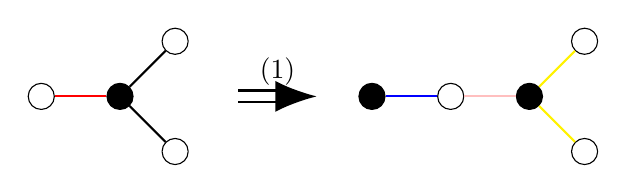
\begin{tikzpicture}
        \begin{scope}[xshift=-2cm]
            \node[circle,draw,fill] (A) at (0, 0) {};
            \node[circle,draw] (B) at (-1,0) {};
            \node[circle,draw] (C) at (0.7,0.7) {};
            \node[circle,draw] (D) at (0.7,-0.7) {};
            
            \draw[thick,red] (A) -- (B);
            \draw[thick] (A) -- (C);
            \draw[thick] (A) -- (D);
        \end{scope}
    
        \draw [line width=1pt, double distance=3pt, arrows = {-Latex[length=0pt 3 0]}] (-0.5,0) -- node[above] {(1)} (0.5,0);
        
        \begin{scope}[xshift=3.2cm]
            \node[circle,draw,fill] (A) at (0, 0) {};
            \node[circle,draw] (B) at (-1,0) {};
            \node[circle,draw] (C) at (0.7,0.7) {};
            \node[circle,draw] (D) at (0.7,-0.7) {};
            \node[circle,draw,fill] (E) at (-2,0) {};
            
            \draw[thick,pink] (A) -- (B);
            \draw[thick,yellow] (A) -- (C);
            \draw[thick,yellow] (A) -- (D);
            \draw[thick,blue] (B) -- (E);
        \end{scope}
    \end{tikzpicture}
\end{center}

This rule will start our algorithm by initializing the counter to one (the blue edge), and marking the two neighboring edges ready for exploration (yellow).

\begin{center}
    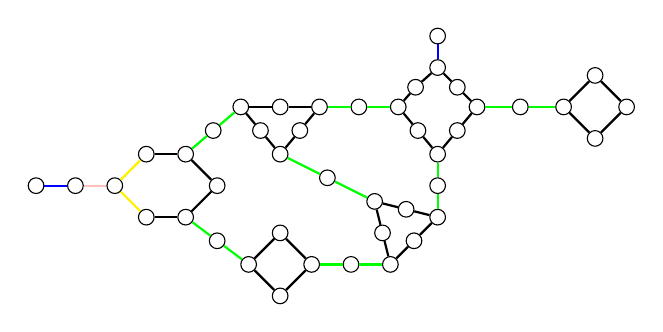
\begin{tikzpicture}
        \node[circle,draw,inner sep=2pt] (v00) at (-0.2,0.6) {};
        \node[circle,draw,inner sep=2pt] (v01) at (-0.2,1.4) {};
        \node[circle,draw,inner sep=2pt] (v02) at (-0.7,1.4) {};
        \node[circle,draw,inner sep=2pt] (v03) at (0.2,1) {};
        \node[circle,draw,inner sep=2pt] (v04) at (-0.7,0.6) {};
        \node[circle,draw,inner sep=2pt] (v05) at (-1.1,1) {};

        \node[circle,draw,inner sep=2pt] (n1) at (-2.1,1) {};
        \node[circle,draw,inner sep=2pt] (s) at (-1.6,1) {};

        \node[circle,draw,inner sep=2pt] (c01) at (0.15,1.7) {};

        \node[circle,draw,inner sep=2pt] (v10) at (0.5,2) {};
        \node[circle,draw,inner sep=2pt] (v11) at (1,1.4) {};
        \node[circle,draw,inner sep=2pt] (v12) at (1.5,2) {};
        \node[circle,draw,inner sep=2pt] (v13) at (0.75,1.7) {};
        \node[circle,draw,inner sep=2pt] (v14) at (1.25,1.7) {};
        \node[circle,draw,inner sep=2pt] (v15) at (1,2) {};

        \node[circle,draw,inner sep=2pt] (c02) at (0.2,0.3) {};

        \node[circle,draw,inner sep=2pt] (v20) at (0.6,0) {};
        \node[circle,draw,inner sep=2pt] (v21) at (1.4,0) {};
        \node[circle,draw,inner sep=2pt] (v22) at (1,-0.4) {};
        \node[circle,draw,inner sep=2pt] (v23) at (1,0.4) {};

        \node[circle,draw,inner sep=2pt] (c13) at (2,2) {};

        \node[circle,draw,inner sep=2pt] (v30) at (2.5,2) {};
        \node[circle,draw,inner sep=2pt] (v31) at (3,1.4) {};
        \node[circle,draw,inner sep=2pt] (v32) at (3.5,2) {};
        \node[circle,draw,inner sep=2pt] (v33) at (2.75,1.7) {};
        \node[circle,draw,inner sep=2pt] (v34) at (3.25,1.7) {};
        \node[circle,draw,inner sep=2pt] (v35) at (3.25,2.25) {};
        \node[circle,draw,inner sep=2pt] (v36) at (3,2.5) {};
        \node[circle,draw,inner sep=2pt] (v37) at (2.72,2.25) {};

        \node[circle,draw,inner sep=2pt] (g) at (3,2.9) {};

        \node[circle,draw,inner sep=2pt] (c14) at (1.6,1.1) {};
        \node[circle,draw,inner sep=2pt] (c24) at (1.9,0) {};
        \node[circle,draw,inner sep=2pt] (c34) at (3,1) {};
    
        \node[circle,draw,inner sep=2pt] (v40) at (2.4,0) {};
        \node[circle,draw,inner sep=2pt] (v41) at (2.2,0.8) {};
        \node[circle,draw,inner sep=2pt] (v42) at (3,0.6) {};
        \node[circle,draw,inner sep=2pt] (v43) at (2.3,0.4) {};
        \node[circle,draw,inner sep=2pt] (v44) at (2.6,0.7) {};
        \node[circle,draw,inner sep=2pt] (v45) at (2.7,0.3) {};
        
        \node[circle,draw,inner sep=2pt] (c35) at (4.05,2) {};

        \node[circle,draw,inner sep=2pt] (v50) at (5,1.6) {};
        \node[circle,draw,inner sep=2pt] (v51) at (5,2.4) {};
        \node[circle,draw,inner sep=2pt] (v52) at (4.6,2) {};
        \node[circle,draw,inner sep=2pt] (v53) at (5.4,2) {};

        \draw[thick,pink] (s) to (v05);
        \draw[thick,blue] (n1) to (s);

        \draw[thick] (v00) to (v04);
        \draw[thick,yellow] (v05) to (v04);
        \draw[thick,yellow] (v02) to (v05);
        \draw[thick] (v02) to (v01);
        \draw[thick] (v01) to (v03);
        \draw[thick] (v03) to (v00);

        \draw[thick] (v10) to (v13);
        \draw[thick] (v13) to (v11);
        \draw[thick] (v11) to (v14);
        \draw[thick] (v14) to (v12);
        \draw[thick] (v12) to (v15);
        \draw[thick] (v15) to (v10);

        \draw[thick] (v20) to (v22);
        \draw[thick] (v22) to (v21);
        \draw[thick] (v21) to (v23);
        \draw[thick] (v23) to (v20);

        \draw[thick] (v30) to (v33);
        \draw[thick] (v33) to (v31);
        \draw[thick] (v31) to (v34);
        \draw[thick] (v34) to (v32);
        \draw[thick] (v32) to (v35);
        \draw[thick] (v35) to (v36);
        \draw[thick] (v36) to (v37);
        \draw[thick] (v37) to (v30);

        \draw[thick, blue] (v36) to (g);

        \draw[thick] (v40) to (v43);
        \draw[thick] (v43) to (v41);
        \draw[thick] (v41) to (v44);
        \draw[thick] (v44) to (v42);
        \draw[thick] (v42) to (v45);
        \draw[thick] (v45) to (v40);

        \draw[thick] (v50) to (v52);
        \draw[thick] (v52) to (v51);
        \draw[thick] (v51) to (v53);
        \draw[thick] (v53) to (v50);

        \draw[thick,green] (v00) -- (c02);
        \draw[thick,green] (c02) -- (v20);

        \draw[thick,green] (v01) -- (c01);
        \draw[thick,green] (c01) -- (v10);

        \draw[thick,green] (v12) -- (c13);
        \draw[thick,green] (c13) -- (v30);

        \draw[thick,green] (v11) -- (c14);
        \draw[thick,green] (c14) -- (v41);

        \draw[thick,green] (v21) -- (c24);
        \draw[thick,green] (c24) -- (v40);

        \draw[thick,green] (v31) -- (c34);
        \draw[thick,green] (c34) -- (v42);

        \draw[thick,green] (v32) -- (c35);
        \draw[thick,green] (c35) -- (v52);
    \end{tikzpicture}
\end{center}

Then we use the following rules to go through all black edges and whenever we reach a green edge we change it to dark green.
This is done so that in the next iteration, we know we already visited that edge once and can now explore the neighboring vertex.

\begin{center}
    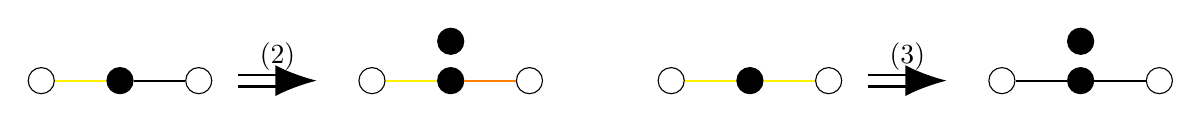
\begin{tikzpicture}
        % SplitRule(
        %     name="Propagate update",
        %     input={"yellow": 1, "black": 1},
        %     node1_connection={"yellow": "yellow", "black": "orange"},
        %     node2_connection={},
        % ),
        \begin{scope}[xshift=-4cm]
            \begin{scope}[xshift=-2cm]
                \node[circle,draw,fill] (A) at (0, 0) {};
                \node[circle,draw] (B) at (-1,0) {};
                \node[circle,draw] (D) at (1,0) {};
                
                \draw[thick,yellow] (A) -- (B);
                \draw[thick,black] (A) -- (D);
            \end{scope}
        
            \draw [line width=1pt, double distance=3pt, arrows = {-Latex[length=0pt 3 0]}] (-0.5,0) -- node[above] {(2)} (0.5,0);
            
            \begin{scope}[xshift=2.2cm]
                \node[circle,draw,fill] (A) at (0, 0) {};
                \node[circle,draw,fill] (A') at (0, 0.5) {};
                \node[circle,draw] (B) at (-1,0) {};
                \node[circle,draw] (D) at (1,0) {};
                
                \draw[thick,yellow] (A) -- (B);
                \draw[thick,orange] (A) -- (D);
            \end{scope}
        \end{scope}

        % SplitRule(
        %     name="Colliding updated",
        %     input={"yellow": 2},
        %     node1_connection={"yellow": "black"},
        %     node2_connection={},
        % ),
        \begin{scope}[xshift=4cm]
            \begin{scope}[xshift=-2cm]
                \node[circle,draw,fill] (A) at (0, 0) {};
                \node[circle,draw] (B) at (-1,0) {};
                \node[circle,draw] (D) at (1,0) {};
                
                \draw[thick,yellow] (A) -- (B);
                \draw[thick,yellow] (A) -- (D);
            \end{scope}
        
            \draw [line width=1pt, double distance=3pt, arrows = {-Latex[length=0pt 3 0]}] (-0.5,0) -- node[above] {(3)} (0.5,0);
            
            \begin{scope}[xshift=2.2cm]
                \node[circle,draw,fill] (A) at (0, 0) {};
                \node[circle,draw,fill] (A') at (0, 0.5) {};
                \node[circle,draw] (B) at (-1,0) {};
                \node[circle,draw] (D) at (1,0) {};
                
                \draw[thick,black] (A) -- (B);
                \draw[thick,black] (A) -- (D);
            \end{scope}
        \end{scope}
    \end{tikzpicture}

    \vspace*{0.5cm}

    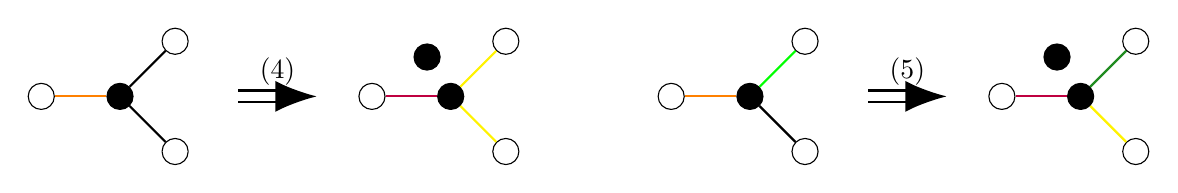
\begin{tikzpicture}
        % SplitRule(
        %     name="Update next nodes",
        %     input={"orange": 1, "black": 2},
        %     node1_connection={"orange": "purple", "black": "yellow"},
        %     node2_connection={},
        % ),
        \begin{scope}[xshift=-4cm]
            \begin{scope}[xshift=-2cm]
                \node[circle,draw,fill] (A) at (0, 0) {};
                \node[circle,draw] (B) at (-1,0) {};
                \node[circle,draw] (C) at (0.7,0.7) {};
                \node[circle,draw] (D) at (0.7,-0.7) {};
                
                \draw[thick,orange] (A) -- (B);
                \draw[thick,black] (A) -- (C);
                \draw[thick,black] (A) -- (D);
            \end{scope}
        
            \draw [line width=1pt, double distance=3pt, arrows = {-Latex[length=0pt 3 0]}] (-0.5,0) -- node[above] {(4)} (0.5,0);
            
            \begin{scope}[xshift=2.2cm]
                \node[circle,draw,fill] (A') at (-0.3, 0.5) {};
                \node[circle,draw,fill] (A) at (0, 0) {};
                \node[circle,draw] (B) at (-1,0) {};
                \node[circle,draw] (C) at (0.7,0.7) {};
                \node[circle,draw] (D) at (0.7,-0.7) {};
                
                \draw[thick,purple] (A) -- (B);
                \draw[thick,yellow] (A) -- (C);
                \draw[thick,yellow] (A) -- (D);
            \end{scope}
        \end{scope}

        % SplitRule(
        %     name="Expand reach",
        %     input={"orange": 1, "green": 1, "black": 1},
        %     node1_connection={"orange": "purple", "green": "lime", "black": "yellow"},
        %     node2_connection={},
        % ),
        \begin{scope}[xshift=4cm]
            \begin{scope}[xshift=-2cm]
                \node[circle,draw,fill] (A) at (0, 0) {};
                \node[circle,draw] (B) at (-1,0) {};
                \node[circle,draw] (C) at (0.7,0.7) {};
                \node[circle,draw] (D) at (0.7,-0.7) {};
                
                \draw[thick,orange] (A) -- (B);
                \draw[thick,green] (A) -- (C);
                \draw[thick,black] (A) -- (D);
            \end{scope}
        
            \draw [line width=1pt, double distance=3pt, arrows = {-Latex[length=0pt 3 0]}] (-0.5,0) -- node[above] {(5)} (0.5,0);
            
            \begin{scope}[xshift=2.2cm]
                \node[circle,draw,fill] (A') at (-0.3, 0.5) {};
                \node[circle,draw,fill] (A) at (0, 0) {};
                \node[circle,draw] (B) at (-1,0) {};
                \node[circle,draw] (C) at (0.7,0.7) {};
                \node[circle,draw] (D) at (0.7,-0.7) {};
                
                \draw[thick,purple] (A) -- (B);
                \draw[thick,forestgreen] (A) -- (C);
                \draw[thick,yellow] (A) -- (D);
            \end{scope}
        \end{scope}
    \end{tikzpicture}

    \vspace*{0.5cm}

    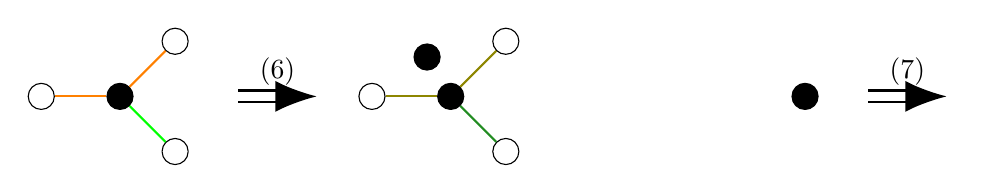
\begin{tikzpicture}
        % SplitRule(
        %     name="Expand reach",
        %     input={"orange": 2, "green": 1},
        %     node1_connection={"orange": "olive", "green": "lime"},
        %     node2_connection={},
        % ),
        \begin{scope}[xshift=-4cm]
            \begin{scope}[xshift=-2cm]
                \node[circle,draw,fill] (A) at (0, 0) {};
                \node[circle,draw] (B) at (-1,0) {};
                \node[circle,draw] (C) at (0.7,0.7) {};
                \node[circle,draw] (D) at (0.7,-0.7) {};
                
                \draw[thick,orange] (A) -- (B);
                \draw[thick,orange] (A) -- (C);
                \draw[thick,green] (A) -- (D);
            \end{scope}
        
            \draw [line width=1pt, double distance=3pt, arrows = {-Latex[length=0pt 3 0]}] (-0.5,0) -- node[above] {(6)} (0.5,0);
            
            \begin{scope}[xshift=2.2cm]
                \node[circle,draw,fill] (A') at (-0.3, 0.5) {};
                \node[circle,draw,fill] (A) at (0, 0) {};
                \node[circle,draw] (B) at (-1,0) {};
                \node[circle,draw] (C) at (0.7,0.7) {};
                \node[circle,draw] (D) at (0.7,-0.7) {};
                
                \draw[thick,olive] (A) -- (B);
                \draw[thick,olive] (A) -- (C);
                \draw[thick,forestgreen] (A) -- (D);
            \end{scope}
        \end{scope}

        % DeleteRule
        \begin{scope}[xshift=4cm]
            \begin{scope}[xshift=-1.3cm]
                \node[circle,draw,fill] (A) at (0, 0) {};
            \end{scope}
        
            \draw [line width=1pt, double distance=3pt, arrows = {-Latex[length=0pt 3 0]}] (-0.5,0) -- node[above] {(7)} (0.5,0);
            
            \begin{scope}[xshift=2.2cm]
            \end{scope}
        \end{scope}
    \end{tikzpicture}
\end{center}

Applying these rules allows us to explore the first ring (vertex u).
We alternate yellow and orange so we know from which edge we reached a node (the one marked with orange).
After an orange edge has been created we update the neighboring edges with yellow to expore them (rule (2) and (4)).
If we reach a green edge we don't traverse it yet but mark it with dark green so we know that in the next iteration we can traverse it (rule (5)).
In those 3 rules we will only change the orange edge to a purple one to remember that this vertex has already been updated.
It might happen that a vertex get updated by two sides at the same time.
It these are the only two edges of the node (rule (3)) then we change the edges back to black basically marking them as done.
If there is also a a green edge (rule (6)), we again change the green edge to dark green, but now instead of turning the orange edges purple we turn them to olive.a
This is just an optimisation as olive will mark that the node and all its children are done updating.
Rule (7) just deletes any isolated vertex we generate with the other Split Rules.

When we apply these rules to our example it depends slightly on which order we apply them but it will turn out that it won't matter in the end.
A resulting graph could be like the following.

\begin{center}
    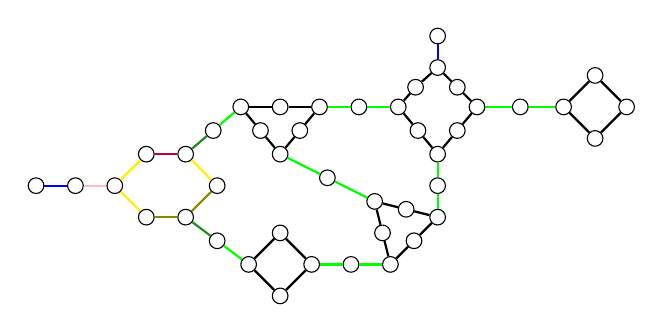
\begin{tikzpicture}
        \node[circle,draw,inner sep=2pt] (v00) at (-0.2,0.6) {};
        \node[circle,draw,inner sep=2pt] (v01) at (-0.2,1.4) {};
        \node[circle,draw,inner sep=2pt] (v02) at (-0.7,1.4) {};
        \node[circle,draw,inner sep=2pt] (v03) at (0.2,1) {};
        \node[circle,draw,inner sep=2pt] (v04) at (-0.7,0.6) {};
        \node[circle,draw,inner sep=2pt] (v05) at (-1.1,1) {};

        \node[circle,draw,inner sep=2pt] (n1) at (-2.1,1) {};
        \node[circle,draw,inner sep=2pt] (s) at (-1.6,1) {};

        \node[circle,draw,inner sep=2pt] (c01) at (0.15,1.7) {};

        \node[circle,draw,inner sep=2pt] (v10) at (0.5,2) {};
        \node[circle,draw,inner sep=2pt] (v11) at (1,1.4) {};
        \node[circle,draw,inner sep=2pt] (v12) at (1.5,2) {};
        \node[circle,draw,inner sep=2pt] (v13) at (0.75,1.7) {};
        \node[circle,draw,inner sep=2pt] (v14) at (1.25,1.7) {};
        \node[circle,draw,inner sep=2pt] (v15) at (1,2) {};

        \node[circle,draw,inner sep=2pt] (c02) at (0.2,0.3) {};

        \node[circle,draw,inner sep=2pt] (v20) at (0.6,0) {};
        \node[circle,draw,inner sep=2pt] (v21) at (1.4,0) {};
        \node[circle,draw,inner sep=2pt] (v22) at (1,-0.4) {};
        \node[circle,draw,inner sep=2pt] (v23) at (1,0.4) {};

        \node[circle,draw,inner sep=2pt] (c13) at (2,2) {};

        \node[circle,draw,inner sep=2pt] (v30) at (2.5,2) {};
        \node[circle,draw,inner sep=2pt] (v31) at (3,1.4) {};
        \node[circle,draw,inner sep=2pt] (v32) at (3.5,2) {};
        \node[circle,draw,inner sep=2pt] (v33) at (2.75,1.7) {};
        \node[circle,draw,inner sep=2pt] (v34) at (3.25,1.7) {};
        \node[circle,draw,inner sep=2pt] (v35) at (3.25,2.25) {};
        \node[circle,draw,inner sep=2pt] (v36) at (3,2.5) {};
        \node[circle,draw,inner sep=2pt] (v37) at (2.72,2.25) {};

        \node[circle,draw,inner sep=2pt] (g) at (3,2.9) {};

        \node[circle,draw,inner sep=2pt] (c14) at (1.6,1.1) {};
        \node[circle,draw,inner sep=2pt] (c24) at (1.9,0) {};
        \node[circle,draw,inner sep=2pt] (c34) at (3,1) {};
    
        \node[circle,draw,inner sep=2pt] (v40) at (2.4,0) {};
        \node[circle,draw,inner sep=2pt] (v41) at (2.2,0.8) {};
        \node[circle,draw,inner sep=2pt] (v42) at (3,0.6) {};
        \node[circle,draw,inner sep=2pt] (v43) at (2.3,0.4) {};
        \node[circle,draw,inner sep=2pt] (v44) at (2.6,0.7) {};
        \node[circle,draw,inner sep=2pt] (v45) at (2.7,0.3) {};
        
        \node[circle,draw,inner sep=2pt] (c35) at (4.05,2) {};

        \node[circle,draw,inner sep=2pt] (v50) at (5,1.6) {};
        \node[circle,draw,inner sep=2pt] (v51) at (5,2.4) {};
        \node[circle,draw,inner sep=2pt] (v52) at (4.6,2) {};
        \node[circle,draw,inner sep=2pt] (v53) at (5.4,2) {};

        \draw[thick,pink] (s) to (v05);
        \draw[thick,blue] (n1) to (s);

        \draw[thick,olive] (v00) to (v04);
        \draw[thick,yellow] (v05) to (v04);
        \draw[thick,yellow] (v02) to (v05);
        \draw[thick,purple] (v02) to (v01);
        \draw[thick,yellow] (v01) to (v03);
        \draw[thick,olive] (v03) to (v00);

        \draw[thick] (v10) to (v13);
        \draw[thick] (v13) to (v11);
        \draw[thick] (v11) to (v14);
        \draw[thick] (v14) to (v12);
        \draw[thick] (v12) to (v15);
        \draw[thick] (v15) to (v10);

        \draw[thick] (v20) to (v22);
        \draw[thick] (v22) to (v21);
        \draw[thick] (v21) to (v23);
        \draw[thick] (v23) to (v20);

        \draw[thick] (v30) to (v33);
        \draw[thick] (v33) to (v31);
        \draw[thick] (v31) to (v34);
        \draw[thick] (v34) to (v32);
        \draw[thick] (v32) to (v35);
        \draw[thick] (v35) to (v36);
        \draw[thick] (v36) to (v37);
        \draw[thick] (v37) to (v30);

        \draw[thick, blue] (v36) to (g);

        \draw[thick] (v40) to (v43);
        \draw[thick] (v43) to (v41);
        \draw[thick] (v41) to (v44);
        \draw[thick] (v44) to (v42);
        \draw[thick] (v42) to (v45);
        \draw[thick] (v45) to (v40);

        \draw[thick] (v50) to (v52);
        \draw[thick] (v52) to (v51);
        \draw[thick] (v51) to (v53);
        \draw[thick] (v53) to (v50);

        \draw[thick,forestgreen] (v00) -- (c02);
        \draw[thick,green] (c02) -- (v20);

        \draw[thick,forestgreen] (v01) -- (c01);
        \draw[thick,green] (c01) -- (v10);

        \draw[thick,green] (v12) -- (c13);
        \draw[thick,green] (c13) -- (v30);

        \draw[thick,green] (v11) -- (c14);
        \draw[thick,green] (c14) -- (v41);

        \draw[thick,green] (v21) -- (c24);
        \draw[thick,green] (c24) -- (v40);

        \draw[thick,green] (v31) -- (c34);
        \draw[thick,green] (c34) -- (v42);

        \draw[thick,green] (v32) -- (c35);
        \draw[thick,green] (c35) -- (v52);
    \end{tikzpicture}
\end{center}

This iteration explored all vertices that have distance 0 from $u$, namely, just the ring of $u$.
We will now want to backtrace all our expored edges to set up the graph for the next iteration.
For this we will need the following rules.

\begin{center}
    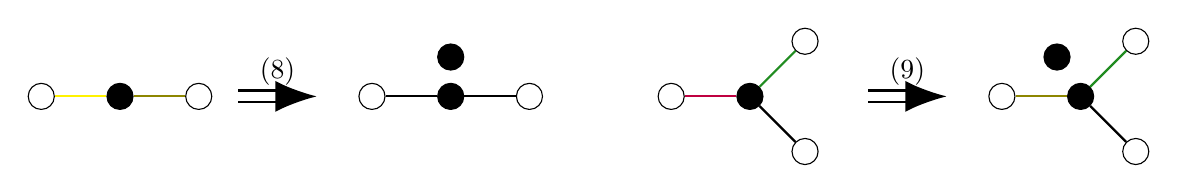
\begin{tikzpicture}
        % SplitRule(
        %     name="Backtrace edge",
        %     input={"yellow": 1, "olive": 1},
        %     node1_connection={"yellow": "black", "olive": "black"},
        %     node2_connection={},
        % ),
        \begin{scope}[xshift=-4cm]
            \begin{scope}[xshift=-2cm]
                \node[circle,draw,fill] (A) at (0, 0) {};
                \node[circle,draw] (B) at (-1,0) {};
                \node[circle,draw] (D) at (1,0) {};
                
                \draw[thick,yellow] (A) -- (B);
                \draw[thick,olive] (A) -- (D);
            \end{scope}
        
            \draw [line width=1pt, double distance=3pt, arrows = {-Latex[length=0pt 3 0]}] (-0.5,0) -- node[above] {(8)} (0.5,0);
            
            \begin{scope}[xshift=2.2cm]
                \node[circle,draw,fill] (A) at (0, 0) {};
                \node[circle,draw,fill] (A') at (0, 0.5) {};
                \node[circle,draw] (B) at (-1,0) {};
                \node[circle,draw] (D) at (1,0) {};
                
                \draw[thick,black] (A) -- (B);
                \draw[thick,black] (A) -- (D);
            \end{scope}
        \end{scope}

        % SplitRule(
        %     name="Done updating (4)",
        %     input={"black": 1, "purple": 1, "lime": 1},
        %     node1_connection={"black": "black", "purple": "olive", "lime": "lime"},
        %     node2_connection={},
        % ),
        \begin{scope}[xshift=4cm]
            \begin{scope}[xshift=-2cm]
                \node[circle,draw,fill] (A) at (0, 0) {};
                \node[circle,draw] (B) at (-1,0) {};
                \node[circle,draw] (C) at (0.7,0.7) {};
                \node[circle,draw] (D) at (0.7,-0.7) {};
                
                \draw[thick,purple] (A) -- (B);
                \draw[thick,forestgreen] (A) -- (C);
                \draw[thick,black] (A) -- (D);
            \end{scope}
        
            \draw [line width=1pt, double distance=3pt, arrows = {-Latex[length=0pt 3 0]}] (-0.5,0) -- node[above] {(9)} (0.5,0);
            
            \begin{scope}[xshift=2.2cm]
                \node[circle,draw,fill] (A') at (-0.3, 0.5) {};
                \node[circle,draw,fill] (A) at (0, 0) {};
                \node[circle,draw] (B) at (-1,0) {};
                \node[circle,draw] (C) at (0.7,0.7) {};
                \node[circle,draw] (D) at (0.7,-0.7) {};
                
                \draw[thick,olive] (A) -- (B);
                \draw[thick,forestgreen] (A) -- (C);
                \draw[thick,black] (A) -- (D);
            \end{scope}
        \end{scope}
    \end{tikzpicture}
\end{center}

These two rules will backtrace the explored vertices and after applying them to our example graph we will get the following graph.

\begin{center}
    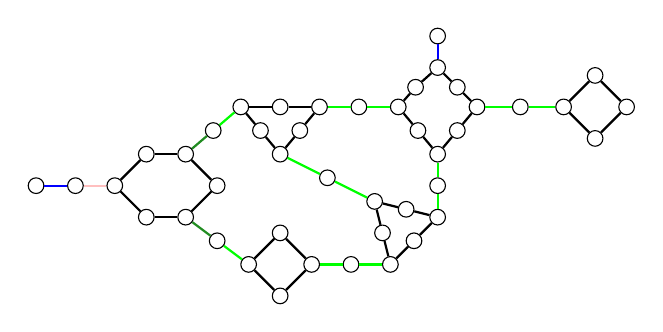
\begin{tikzpicture}
        \node[circle,draw,inner sep=2pt] (v00) at (-0.2,0.6) {};
        \node[circle,draw,inner sep=2pt] (v01) at (-0.2,1.4) {};
        \node[circle,draw,inner sep=2pt] (v02) at (-0.7,1.4) {};
        \node[circle,draw,inner sep=2pt] (v03) at (0.2,1) {};
        \node[circle,draw,inner sep=2pt] (v04) at (-0.7,0.6) {};
        \node[circle,draw,inner sep=2pt] (v05) at (-1.1,1) {};

        \node[circle,draw,inner sep=2pt] (n1) at (-2.1,1) {};
        \node[circle,draw,inner sep=2pt] (s) at (-1.6,1) {};

        \node[circle,draw,inner sep=2pt] (c01) at (0.15,1.7) {};

        \node[circle,draw,inner sep=2pt] (v10) at (0.5,2) {};
        \node[circle,draw,inner sep=2pt] (v11) at (1,1.4) {};
        \node[circle,draw,inner sep=2pt] (v12) at (1.5,2) {};
        \node[circle,draw,inner sep=2pt] (v13) at (0.75,1.7) {};
        \node[circle,draw,inner sep=2pt] (v14) at (1.25,1.7) {};
        \node[circle,draw,inner sep=2pt] (v15) at (1,2) {};

        \node[circle,draw,inner sep=2pt] (c02) at (0.2,0.3) {};

        \node[circle,draw,inner sep=2pt] (v20) at (0.6,0) {};
        \node[circle,draw,inner sep=2pt] (v21) at (1.4,0) {};
        \node[circle,draw,inner sep=2pt] (v22) at (1,-0.4) {};
        \node[circle,draw,inner sep=2pt] (v23) at (1,0.4) {};

        \node[circle,draw,inner sep=2pt] (c13) at (2,2) {};

        \node[circle,draw,inner sep=2pt] (v30) at (2.5,2) {};
        \node[circle,draw,inner sep=2pt] (v31) at (3,1.4) {};
        \node[circle,draw,inner sep=2pt] (v32) at (3.5,2) {};
        \node[circle,draw,inner sep=2pt] (v33) at (2.75,1.7) {};
        \node[circle,draw,inner sep=2pt] (v34) at (3.25,1.7) {};
        \node[circle,draw,inner sep=2pt] (v35) at (3.25,2.25) {};
        \node[circle,draw,inner sep=2pt] (v36) at (3,2.5) {};
        \node[circle,draw,inner sep=2pt] (v37) at (2.72,2.25) {};

        \node[circle,draw,inner sep=2pt] (g) at (3,2.9) {};

        \node[circle,draw,inner sep=2pt] (c14) at (1.6,1.1) {};
        \node[circle,draw,inner sep=2pt] (c24) at (1.9,0) {};
        \node[circle,draw,inner sep=2pt] (c34) at (3,1) {};
    
        \node[circle,draw,inner sep=2pt] (v40) at (2.4,0) {};
        \node[circle,draw,inner sep=2pt] (v41) at (2.2,0.8) {};
        \node[circle,draw,inner sep=2pt] (v42) at (3,0.6) {};
        \node[circle,draw,inner sep=2pt] (v43) at (2.3,0.4) {};
        \node[circle,draw,inner sep=2pt] (v44) at (2.6,0.7) {};
        \node[circle,draw,inner sep=2pt] (v45) at (2.7,0.3) {};
        
        \node[circle,draw,inner sep=2pt] (c35) at (4.05,2) {};

        \node[circle,draw,inner sep=2pt] (v50) at (5,1.6) {};
        \node[circle,draw,inner sep=2pt] (v51) at (5,2.4) {};
        \node[circle,draw,inner sep=2pt] (v52) at (4.6,2) {};
        \node[circle,draw,inner sep=2pt] (v53) at (5.4,2) {};

        \draw[thick,pink] (s) to (v05);
        \draw[thick,blue] (n1) to (s);

        \draw[thick] (v00) to (v04);
        \draw[thick] (v05) to (v04);
        \draw[thick] (v02) to (v05);
        \draw[thick] (v02) to (v01);
        \draw[thick] (v01) to (v03);
        \draw[thick] (v03) to (v00);

        \draw[thick] (v10) to (v13);
        \draw[thick] (v13) to (v11);
        \draw[thick] (v11) to (v14);
        \draw[thick] (v14) to (v12);
        \draw[thick] (v12) to (v15);
        \draw[thick] (v15) to (v10);

        \draw[thick] (v20) to (v22);
        \draw[thick] (v22) to (v21);
        \draw[thick] (v21) to (v23);
        \draw[thick] (v23) to (v20);

        \draw[thick] (v30) to (v33);
        \draw[thick] (v33) to (v31);
        \draw[thick] (v31) to (v34);
        \draw[thick] (v34) to (v32);
        \draw[thick] (v32) to (v35);
        \draw[thick] (v35) to (v36);
        \draw[thick] (v36) to (v37);
        \draw[thick] (v37) to (v30);

        \draw[thick, blue] (v36) to (g);

        \draw[thick] (v40) to (v43);
        \draw[thick] (v43) to (v41);
        \draw[thick] (v41) to (v44);
        \draw[thick] (v44) to (v42);
        \draw[thick] (v42) to (v45);
        \draw[thick] (v45) to (v40);

        \draw[thick] (v50) to (v52);
        \draw[thick] (v52) to (v51);
        \draw[thick] (v51) to (v53);
        \draw[thick] (v53) to (v50);

        \draw[thick,forestgreen] (v00) -- (c02);
        \draw[thick,green] (c02) -- (v20);

        \draw[thick,forestgreen] (v01) -- (c01);
        \draw[thick,green] (c01) -- (v10);

        \draw[thick,green] (v12) -- (c13);
        \draw[thick,green] (c13) -- (v30);

        \draw[thick,green] (v11) -- (c14);
        \draw[thick,green] (c14) -- (v41);

        \draw[thick,green] (v21) -- (c24);
        \draw[thick,green] (c24) -- (v40);

        \draw[thick,green] (v31) -- (c34);
        \draw[thick,green] (c34) -- (v42);

        \draw[thick,green] (v32) -- (c35);
        \draw[thick,green] (c35) -- (v52);
    \end{tikzpicture}
\end{center}

As you can see, we now almost have the original graph back but have accomplished the following tasks:
\begin{itemize}
    \item Initialize counter (blue edge) to one
    \item Visit all green edges that can be reached from $u$ in 0 steps and marked them with dark green
\end{itemize}

We will know continue doing this.
First to start the second round we need new rules to increament the counter by one.

\begin{center}
    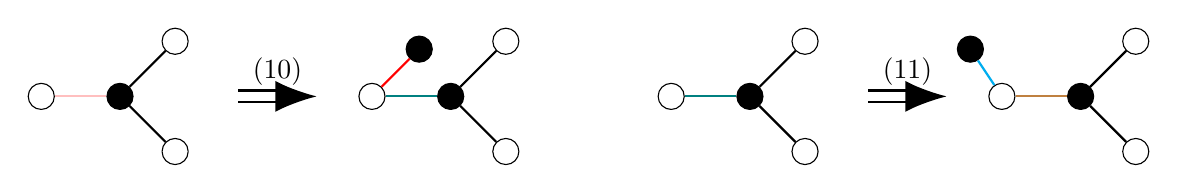
\begin{tikzpicture}
        % SplitRule(
        %     name="Next round (1)",
        %     input={"pink": 1, "black": 2},
        %     node1_connection={"pink": "teal", "black": "black"},
        %     node2_connection={"pink": "red"},
        % ),
        \begin{scope}[xshift=-4cm]
            \begin{scope}[xshift=-2cm]
                \node[circle,draw,fill] (A) at (0, 0) {};
                \node[circle,draw] (B) at (-1,0) {};
                \node[circle,draw] (C) at (0.7,0.7) {};
                \node[circle,draw] (D) at (0.7,-0.7) {};
                
                \draw[thick,pink] (A) -- (B);
                \draw[thick,black] (A) -- (C);
                \draw[thick,black] (A) -- (D);
            \end{scope}
        
            \draw [line width=1pt, double distance=3pt, arrows = {-Latex[length=0pt 3 0]}] (-0.5,0) -- node[above] {(10)} (0.5,0);
            
            \begin{scope}[xshift=2.2cm]
                \node[circle,draw,fill] (A') at (-0.4, 0.6) {};
                \node[circle,draw,fill] (A) at (0, 0) {};
                \node[circle,draw] (B) at (-1,0) {};
                \node[circle,draw] (C) at (0.7,0.7) {};
                \node[circle,draw] (D) at (0.7,-0.7) {};
                
                \draw[thick,teal] (A) -- (B);
                \draw[thick,black] (A) -- (C);
                \draw[thick,black] (A) -- (D);
                \draw[thick,red] (B) -- (A');
            \end{scope}
        \end{scope}

        % SplitRule(
        %     name="Next round (2)",
        %     input={"teal": 1, "black": 2},
        %     node1_connection={"teal": "brown", "black": "black"},
        %     node2_connection={"teal": "cyan"},
        % ),
        \begin{scope}[xshift=4cm]
            \begin{scope}[xshift=-2cm]
                \node[circle,draw,fill] (A) at (0, 0) {};
                \node[circle,draw] (B) at (-1,0) {};
                \node[circle,draw] (C) at (0.7,0.7) {};
                \node[circle,draw] (D) at (0.7,-0.7) {};
                
                \draw[thick,teal] (A) -- (B);
                \draw[thick,black] (A) -- (C);
                \draw[thick,black] (A) -- (D);
            \end{scope}
        
            \draw [line width=1pt, double distance=3pt, arrows = {-Latex[length=0pt 3 0]}] (-0.5,0) -- node[above] {(11)} (0.5,0);
            
            \begin{scope}[xshift=2.2cm]
                \node[circle,draw,fill] (A') at (-1.4, 0.6) {};
                \node[circle,draw,fill] (A) at (0, 0) {};
                \node[circle,draw] (B) at (-1,0) {};
                \node[circle,draw] (C) at (0.7,0.7) {};
                \node[circle,draw] (D) at (0.7,-0.7) {};
                
                \draw[thick,brown] (A) -- (B);
                \draw[thick,black] (A) -- (C);
                \draw[thick,black] (A) -- (D);
                \draw[thick,cyan] (B) -- (A');
            \end{scope}
        \end{scope}
    \end{tikzpicture}

    \vspace*{0.5cm}

    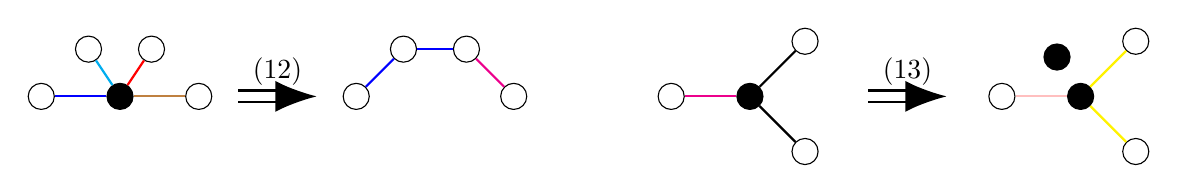
\begin{tikzpicture}
        % DeleteRule(
        %     name="Next round (3)",
        %     input={"brown": 1, "red": 1, "cyan": 1, "blue": 1},
        %     rewiring={("blue", "cyan"): "blue", ("cyan", "red"): "blue", ("red", "brown"): "magenta"},
        % ),
        \begin{scope}[xshift=-4cm]
            \begin{scope}[xshift=-2cm]
                \node[circle,draw,fill] (A) at (0, 0) {};
                \node[circle,draw] (B) at (-1,0) {};
                \node[circle,draw] (C) at (1,0) {};
                \node[circle,draw] (D) at (-0.4,0.6) {};
                \node[circle,draw] (E) at (0.4,0.6) {};
                
                \draw[thick,blue] (A) -- (B);
                \draw[thick,cyan] (A) -- (D);
                \draw[thick,red] (A) -- (E);
                \draw[thick,brown] (A) -- (C);
            \end{scope}
        
            \draw [line width=1pt, double distance=3pt, arrows = {-Latex[length=0pt 3 0]}] (-0.5,0) -- node[above] {(12)} (0.5,0);
            
            \begin{scope}[xshift=2cm]
                \node[circle,draw] (B) at (-1,0) {};
                \node[circle,draw] (C) at (1,0) {};
                \node[circle,draw] (D) at (-0.4,0.6) {};
                \node[circle,draw] (E) at (0.4,0.6) {};
                
                \draw[thick,blue] (B) -- (D);
                \draw[thick,blue] (D) -- (E);
                \draw[thick,magenta] (E) -- (C);
            \end{scope}
        \end{scope}

        % SplitRule(
        %     name="Start update (2)",
        %     input={"magenta": 1, "black": 2},
        %     node1_connection={"magenta": "pink", "black": "yellow"},
        %     node2_connection={},
        % ),
        \begin{scope}[xshift=4cm]
            \begin{scope}[xshift=-2cm]
                \node[circle,draw,fill] (A) at (0, 0) {};
                \node[circle,draw] (B) at (-1,0) {};
                \node[circle,draw] (C) at (0.7,0.7) {};
                \node[circle,draw] (D) at (0.7,-0.7) {};
                
                \draw[thick,magenta] (A) -- (B);
                \draw[thick,black] (A) -- (C);
                \draw[thick,black] (A) -- (D);
            \end{scope}
        
            \draw [line width=1pt, double distance=3pt, arrows = {-Latex[length=0pt 3 0]}] (-0.5,0) -- node[above] {(13)} (0.5,0);
            
            \begin{scope}[xshift=2.2cm]
                \node[circle,draw,fill] (A') at (-0.3, 0.5) {};
                \node[circle,draw,fill] (A) at (0, 0) {};
                \node[circle,draw] (B) at (-1,0) {};
                \node[circle,draw] (C) at (0.7,0.7) {};
                \node[circle,draw] (D) at (0.7,-0.7) {};
                
                \draw[thick,pink] (A) -- (B);
                \draw[thick,yellow] (A) -- (C);
                \draw[thick,yellow] (A) -- (D);
            \end{scope}
        \end{scope}
    \end{tikzpicture}
\end{center}

Rules (10) and (11) first add two new vertices to the start of the counter connected with red and cyan respectively.
Then the Delete Rule (12) rewires the neighboring nodes so that we increament the counter by one (we generate two blue edges) and set the edge to vertex $u$ to magenta.
Rule (13) then start the second iteration by setting the first edges to yellow again.
This result it the following graph.

\begin{center}
    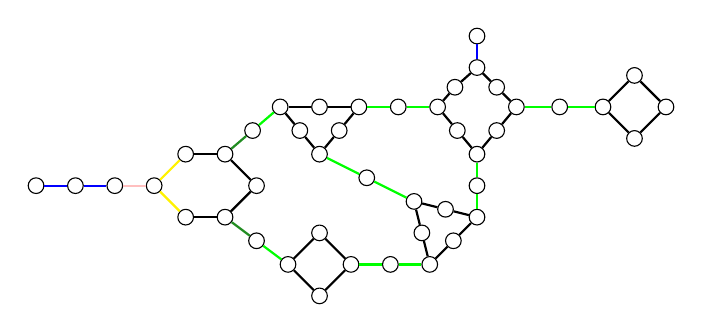
\begin{tikzpicture}
        \node[circle,draw,inner sep=2pt] (v00) at (-0.2,0.6) {};
        \node[circle,draw,inner sep=2pt] (v01) at (-0.2,1.4) {};
        \node[circle,draw,inner sep=2pt] (v02) at (-0.7,1.4) {};
        \node[circle,draw,inner sep=2pt] (v03) at (0.2,1) {};
        \node[circle,draw,inner sep=2pt] (v04) at (-0.7,0.6) {};
        \node[circle,draw,inner sep=2pt] (v05) at (-1.1,1) {};

        \node[circle,draw,inner sep=2pt] (s) at (-1.6,1) {};
        \node[circle,draw,inner sep=2pt] (n1) at (-2.1,1) {};
        \node[circle,draw,inner sep=2pt] (n2) at (-2.6,1) {};

        \node[circle,draw,inner sep=2pt] (c01) at (0.15,1.7) {};

        \node[circle,draw,inner sep=2pt] (v10) at (0.5,2) {};
        \node[circle,draw,inner sep=2pt] (v11) at (1,1.4) {};
        \node[circle,draw,inner sep=2pt] (v12) at (1.5,2) {};
        \node[circle,draw,inner sep=2pt] (v13) at (0.75,1.7) {};
        \node[circle,draw,inner sep=2pt] (v14) at (1.25,1.7) {};
        \node[circle,draw,inner sep=2pt] (v15) at (1,2) {};

        \node[circle,draw,inner sep=2pt] (c02) at (0.2,0.3) {};

        \node[circle,draw,inner sep=2pt] (v20) at (0.6,0) {};
        \node[circle,draw,inner sep=2pt] (v21) at (1.4,0) {};
        \node[circle,draw,inner sep=2pt] (v22) at (1,-0.4) {};
        \node[circle,draw,inner sep=2pt] (v23) at (1,0.4) {};

        \node[circle,draw,inner sep=2pt] (c13) at (2,2) {};

        \node[circle,draw,inner sep=2pt] (v30) at (2.5,2) {};
        \node[circle,draw,inner sep=2pt] (v31) at (3,1.4) {};
        \node[circle,draw,inner sep=2pt] (v32) at (3.5,2) {};
        \node[circle,draw,inner sep=2pt] (v33) at (2.75,1.7) {};
        \node[circle,draw,inner sep=2pt] (v34) at (3.25,1.7) {};
        \node[circle,draw,inner sep=2pt] (v35) at (3.25,2.25) {};
        \node[circle,draw,inner sep=2pt] (v36) at (3,2.5) {};
        \node[circle,draw,inner sep=2pt] (v37) at (2.72,2.25) {};

        \node[circle,draw,inner sep=2pt] (g) at (3,2.9) {};

        \node[circle,draw,inner sep=2pt] (c14) at (1.6,1.1) {};
        \node[circle,draw,inner sep=2pt] (c24) at (1.9,0) {};
        \node[circle,draw,inner sep=2pt] (c34) at (3,1) {};
    
        \node[circle,draw,inner sep=2pt] (v40) at (2.4,0) {};
        \node[circle,draw,inner sep=2pt] (v41) at (2.2,0.8) {};
        \node[circle,draw,inner sep=2pt] (v42) at (3,0.6) {};
        \node[circle,draw,inner sep=2pt] (v43) at (2.3,0.4) {};
        \node[circle,draw,inner sep=2pt] (v44) at (2.6,0.7) {};
        \node[circle,draw,inner sep=2pt] (v45) at (2.7,0.3) {};
        
        \node[circle,draw,inner sep=2pt] (c35) at (4.05,2) {};

        \node[circle,draw,inner sep=2pt] (v50) at (5,1.6) {};
        \node[circle,draw,inner sep=2pt] (v51) at (5,2.4) {};
        \node[circle,draw,inner sep=2pt] (v52) at (4.6,2) {};
        \node[circle,draw,inner sep=2pt] (v53) at (5.4,2) {};

        \draw[thick,pink] (s) to (v05);
        \draw[thick,blue] (n1) to (s);
        \draw[thick,blue] (n2) to (n1);

        \draw[thick] (v00) to (v04);
        \draw[thick,yellow] (v05) to (v04);
        \draw[thick,yellow] (v02) to (v05);
        \draw[thick] (v02) to (v01);
        \draw[thick] (v01) to (v03);
        \draw[thick] (v03) to (v00);

        \draw[thick] (v10) to (v13);
        \draw[thick] (v13) to (v11);
        \draw[thick] (v11) to (v14);
        \draw[thick] (v14) to (v12);
        \draw[thick] (v12) to (v15);
        \draw[thick] (v15) to (v10);

        \draw[thick] (v20) to (v22);
        \draw[thick] (v22) to (v21);
        \draw[thick] (v21) to (v23);
        \draw[thick] (v23) to (v20);

        \draw[thick] (v30) to (v33);
        \draw[thick] (v33) to (v31);
        \draw[thick] (v31) to (v34);
        \draw[thick] (v34) to (v32);
        \draw[thick] (v32) to (v35);
        \draw[thick] (v35) to (v36);
        \draw[thick] (v36) to (v37);
        \draw[thick] (v37) to (v30);

        \draw[thick, blue] (v36) to (g);

        \draw[thick] (v40) to (v43);
        \draw[thick] (v43) to (v41);
        \draw[thick] (v41) to (v44);
        \draw[thick] (v44) to (v42);
        \draw[thick] (v42) to (v45);
        \draw[thick] (v45) to (v40);

        \draw[thick] (v50) to (v52);
        \draw[thick] (v52) to (v51);
        \draw[thick] (v51) to (v53);
        \draw[thick] (v53) to (v50);

        \draw[thick,forestgreen] (v00) -- (c02);
        \draw[thick,green] (c02) -- (v20);

        \draw[thick,forestgreen] (v01) -- (c01);
        \draw[thick,green] (c01) -- (v10);

        \draw[thick,green] (v12) -- (c13);
        \draw[thick,green] (c13) -- (v30);

        \draw[thick,green] (v11) -- (c14);
        \draw[thick,green] (c14) -- (v41);

        \draw[thick,green] (v21) -- (c24);
        \draw[thick,green] (c24) -- (v40);

        \draw[thick,green] (v31) -- (c34);
        \draw[thick,green] (c34) -- (v42);

        \draw[thick,green] (v32) -- (c35);
        \draw[thick,green] (c35) -- (v52);
    \end{tikzpicture}
\end{center}

We now want to explore all green edges that can be reached in 1 steps.
For this we need new rules to traverse the edges we marked with dark green in the previous iteration.

\begin{center}
    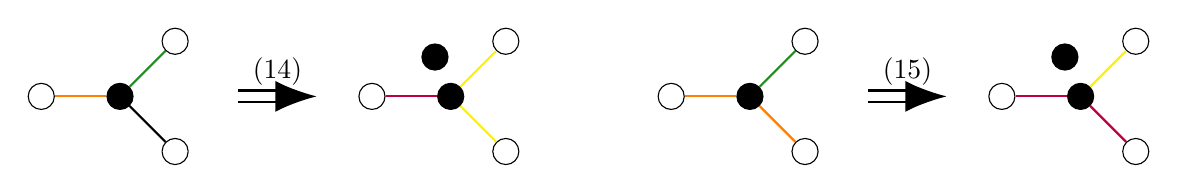
\begin{tikzpicture}
        % SplitRule(
        %     name="Update next nodes (2)",
        %     input={"orange": 1, "black": 1, "lime": 1},
        %     node1_connection={"orange": "purple", "black": "yellow", "lime": "yellow"},
        %     node2_connection={},
        % ),
        \begin{scope}[xshift=-4cm]
            \begin{scope}[xshift=-2cm]
                \node[circle,draw,fill] (A) at (0, 0) {};
                \node[circle,draw] (B) at (-1,0) {};
                \node[circle,draw] (C) at (0.7,0.7) {};
                \node[circle,draw] (D) at (0.7,-0.7) {};
                
                \draw[thick,orange] (A) -- (B);
                \draw[thick,forestgreen] (A) -- (C);
                \draw[thick,black] (A) -- (D);
            \end{scope}
        
            \draw [line width=1pt, double distance=3pt, arrows = {-Latex[length=0pt 3 0]}] (-0.5,0) -- node[above] {(14)} (0.5,0);
            
            \begin{scope}[xshift=2.2cm]
                \node[circle,draw,fill] (A') at (-0.2, 0.5) {};
                \node[circle,draw,fill] (A) at (0, 0) {};
                \node[circle,draw] (B) at (-1,0) {};
                \node[circle,draw] (C) at (0.7,0.7) {};
                \node[circle,draw] (D) at (0.7,-0.7) {};
                
                \draw[thick,purple] (A) -- (B);
                \draw[thick,yellow] (A) -- (C);
                \draw[thick,yellow] (A) -- (D);
            \end{scope}
        \end{scope}

        % SplitRule(
        %     name="Update next nodes (4)",
        %     input={"orange": 2, "lime": 1},
        %     node1_connection={"orange": "purple", "lime": "yellow"},
        %     node2_connection={},
        % ),
        \begin{scope}[xshift=4cm]
            \begin{scope}[xshift=-2cm]
                \node[circle,draw,fill] (A) at (0, 0) {};
                \node[circle,draw] (B) at (-1,0) {};
                \node[circle,draw] (C) at (0.7,0.7) {};
                \node[circle,draw] (D) at (0.7,-0.7) {};
                
                \draw[thick,orange] (A) -- (B);
                \draw[thick,forestgreen] (A) -- (C);
                \draw[thick,orange] (A) -- (D);
            \end{scope}
        
            \draw [line width=1pt, double distance=3pt, arrows = {-Latex[length=0pt 3 0]}] (-0.5,0) -- node[above] {(15)} (0.5,0);
            
            \begin{scope}[xshift=2.2cm]
                \node[circle,draw,fill] (A') at (-0.2, 0.5) {};
                \node[circle,draw,fill] (A) at (0, 0) {};
                \node[circle,draw] (B) at (-1,0) {};
                \node[circle,draw] (C) at (0.7,0.7) {};
                \node[circle,draw] (D) at (0.7,-0.7) {};
                
                \draw[thick,purple] (A) -- (B);
                \draw[thick,yellow] (A) -- (C);
                \draw[thick,purple] (A) -- (D);
            \end{scope}
        \end{scope}
    \end{tikzpicture}

    \vspace*{0.5cm}

    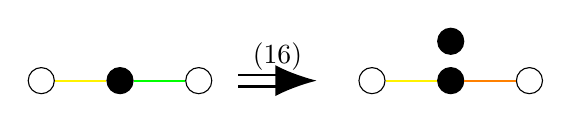
\begin{tikzpicture}
        % SplitRule(
        %     name="Propagate update (new edge)",
        %     input={"yellow": 1, "green": 1},
        %     node1_connection={"yellow": "yellow", "green": "orange"},
        %     node2_connection={},
        % ),
        \begin{scope}[xshift=4cm]
            \begin{scope}[xshift=-2cm]
                \node[circle,draw,fill] (A) at (0, 0) {};
                \node[circle,draw] (B) at (-1,0) {};
                \node[circle,draw] (C) at (1,0) {};
                
                \draw[thick,yellow] (A) -- (B);
                \draw[thick,green] (A) -- (C);
            \end{scope}
        
            \draw [line width=1pt, double distance=3pt, arrows = {-Latex[length=0pt 3 0]}] (-0.5,0) -- node[above] {(16)} (0.5,0);
            
            \begin{scope}[xshift=2.2cm]
                \node[circle,draw,fill] (A') at (0, 0.5) {};
                \node[circle,draw,fill] (A) at (0, 0) {};
                \node[circle,draw] (B) at (-1,0) {};
                \node[circle,draw] (C) at (1,0) {};
                
                \draw[thick,yellow] (A) -- (B);
                \draw[thick,orange] (A) -- (C);
            \end{scope}
        \end{scope}
    \end{tikzpicture}
\end{center}

We might reach a node at a dark green edge from one side (rule (14)) or from two sides at the same time (rule (15)).
Since we already reached the dark green edge last iteration we now change it to yellow so that the neighboring vertex gets explored.
We also make the node as visited (change orange to purple) and explore any unexplored direction (second yellow edge in rule (14)).
Rule (16) then changes the second green edge in the connection the the neighboring vertex to orange.

Applying the rules that we have already introduced might lead to the following graph.

\begin{center}
    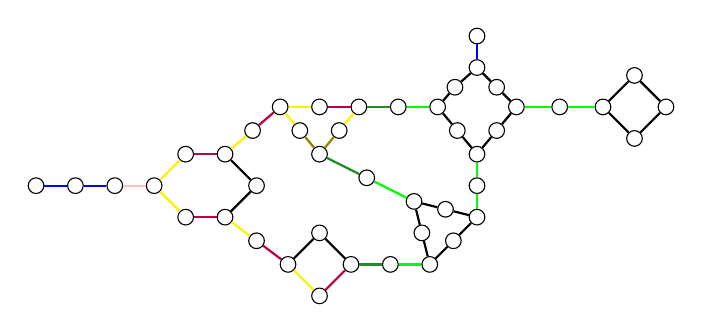
\begin{tikzpicture}
        \node[circle,draw,inner sep=2pt] (v00) at (-0.2,0.6) {};
        \node[circle,draw,inner sep=2pt] (v01) at (-0.2,1.4) {};
        \node[circle,draw,inner sep=2pt] (v02) at (-0.7,1.4) {};
        \node[circle,draw,inner sep=2pt] (v03) at (0.2,1) {};
        \node[circle,draw,inner sep=2pt] (v04) at (-0.7,0.6) {};
        \node[circle,draw,inner sep=2pt] (v05) at (-1.1,1) {};

        \node[circle,draw,inner sep=2pt] (s) at (-1.6,1) {};
        \node[circle,draw,inner sep=2pt] (n1) at (-2.1,1) {};
        \node[circle,draw,inner sep=2pt] (n2) at (-2.6,1) {};

        \node[circle,draw,inner sep=2pt] (c01) at (0.15,1.7) {};

        \node[circle,draw,inner sep=2pt] (v10) at (0.5,2) {};
        \node[circle,draw,inner sep=2pt] (v11) at (1,1.4) {};
        \node[circle,draw,inner sep=2pt] (v12) at (1.5,2) {};
        \node[circle,draw,inner sep=2pt] (v13) at (0.75,1.7) {};
        \node[circle,draw,inner sep=2pt] (v14) at (1.25,1.7) {};
        \node[circle,draw,inner sep=2pt] (v15) at (1,2) {};

        \node[circle,draw,inner sep=2pt] (c02) at (0.2,0.3) {};

        \node[circle,draw,inner sep=2pt] (v20) at (0.6,0) {};
        \node[circle,draw,inner sep=2pt] (v21) at (1.4,0) {};
        \node[circle,draw,inner sep=2pt] (v22) at (1,-0.4) {};
        \node[circle,draw,inner sep=2pt] (v23) at (1,0.4) {};

        \node[circle,draw,inner sep=2pt] (c13) at (2,2) {};

        \node[circle,draw,inner sep=2pt] (v30) at (2.5,2) {};
        \node[circle,draw,inner sep=2pt] (v31) at (3,1.4) {};
        \node[circle,draw,inner sep=2pt] (v32) at (3.5,2) {};
        \node[circle,draw,inner sep=2pt] (v33) at (2.75,1.7) {};
        \node[circle,draw,inner sep=2pt] (v34) at (3.25,1.7) {};
        \node[circle,draw,inner sep=2pt] (v35) at (3.25,2.25) {};
        \node[circle,draw,inner sep=2pt] (v36) at (3,2.5) {};
        \node[circle,draw,inner sep=2pt] (v37) at (2.72,2.25) {};

        \node[circle,draw,inner sep=2pt] (g) at (3,2.9) {};

        \node[circle,draw,inner sep=2pt] (c14) at (1.6,1.1) {};
        \node[circle,draw,inner sep=2pt] (c24) at (1.9,0) {};
        \node[circle,draw,inner sep=2pt] (c34) at (3,1) {};
    
        \node[circle,draw,inner sep=2pt] (v40) at (2.4,0) {};
        \node[circle,draw,inner sep=2pt] (v41) at (2.2,0.8) {};
        \node[circle,draw,inner sep=2pt] (v42) at (3,0.6) {};
        \node[circle,draw,inner sep=2pt] (v43) at (2.3,0.4) {};
        \node[circle,draw,inner sep=2pt] (v44) at (2.6,0.7) {};
        \node[circle,draw,inner sep=2pt] (v45) at (2.7,0.3) {};
        
        \node[circle,draw,inner sep=2pt] (c35) at (4.05,2) {};

        \node[circle,draw,inner sep=2pt] (v50) at (5,1.6) {};
        \node[circle,draw,inner sep=2pt] (v51) at (5,2.4) {};
        \node[circle,draw,inner sep=2pt] (v52) at (4.6,2) {};
        \node[circle,draw,inner sep=2pt] (v53) at (5.4,2) {};

        \draw[thick,pink] (s) to (v05);
        \draw[thick,blue] (n1) to (s);
        \draw[thick,blue] (n2) to (n1);

        \draw[thick,purple] (v00) to (v04);
        \draw[thick,yellow] (v05) to (v04);
        \draw[thick,yellow] (v02) to (v05);
        \draw[thick,purple] (v02) to (v01);
        \draw[thick] (v01) to (v03);
        \draw[thick] (v03) to (v00);

        \draw[thick,yellow] (v10) to (v13);
        \draw[thick,olive] (v13) to (v11);
        \draw[thick,olive] (v11) to (v14);
        \draw[thick,yellow] (v14) to (v12);
        \draw[thick,purple] (v12) to (v15);
        \draw[thick,yellow] (v15) to (v10);

        \draw[thick,yellow] (v20) to (v22);
        \draw[thick,purple] (v22) to (v21);
        \draw[thick] (v21) to (v23);
        \draw[thick] (v23) to (v20);

        \draw[thick] (v30) to (v33);
        \draw[thick] (v33) to (v31);
        \draw[thick] (v31) to (v34);
        \draw[thick] (v34) to (v32);
        \draw[thick] (v32) to (v35);
        \draw[thick] (v35) to (v36);
        \draw[thick] (v36) to (v37);
        \draw[thick] (v37) to (v30);

        \draw[thick, blue] (v36) to (g);

        \draw[thick] (v40) to (v43);
        \draw[thick] (v43) to (v41);
        \draw[thick] (v41) to (v44);
        \draw[thick] (v44) to (v42);
        \draw[thick] (v42) to (v45);
        \draw[thick] (v45) to (v40);

        \draw[thick] (v50) to (v52);
        \draw[thick] (v52) to (v51);
        \draw[thick] (v51) to (v53);
        \draw[thick] (v53) to (v50);

        \draw[thick,yellow] (v00) -- (c02);
        \draw[thick,purple] (c02) -- (v20);

        \draw[thick,yellow] (v01) -- (c01);
        \draw[thick,purple] (c01) -- (v10);

        \draw[thick,forestgreen] (v12) -- (c13);
        \draw[thick,green] (c13) -- (v30);

        \draw[thick,forestgreen] (v11) -- (c14);
        \draw[thick,green] (c14) -- (v41);

        \draw[thick,forestgreen] (v21) -- (c24);
        \draw[thick,green] (c24) -- (v40);

        \draw[thick,green] (v31) -- (c34);
        \draw[thick,green] (c34) -- (v42);

        \draw[thick,green] (v32) -- (c35);
        \draw[thick,green] (c35) -- (v52);
    \end{tikzpicture}
\end{center}

We will now backtrace again might need the following rule where multiple update paths meet.

\begin{center}
    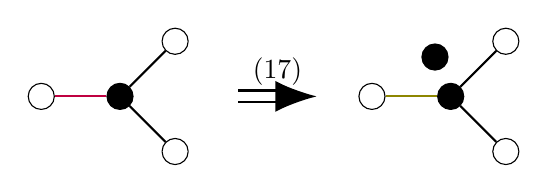
\begin{tikzpicture}
        % SplitRule(
        %     name="Done updating (1)",
        %     input={"black": 2, "purple": 1},
        %     node1_connection={"black": "black", "purple": "olive"},
        %     node2_connection={},
        % ),
        \begin{scope}[xshift=-4cm]
            \begin{scope}[xshift=-2cm]
                \node[circle,draw,fill] (A) at (0, 0) {};
                \node[circle,draw] (B) at (-1,0) {};
                \node[circle,draw] (C) at (0.7,0.7) {};
                \node[circle,draw] (D) at (0.7,-0.7) {};
                
                \draw[thick,purple] (A) -- (B);
                \draw[thick,black] (A) -- (C);
                \draw[thick,black] (A) -- (D);
            \end{scope}
        
            \draw [line width=1pt, double distance=3pt, arrows = {-Latex[length=0pt 3 0]}] (-0.5,0) -- node[above] {(17)} (0.5,0);
            
            \begin{scope}[xshift=2.2cm]
                \node[circle,draw,fill] (A') at (-0.2, 0.5) {};
                \node[circle,draw,fill] (A) at (0, 0) {};
                \node[circle,draw] (B) at (-1,0) {};
                \node[circle,draw] (C) at (0.7,0.7) {};
                \node[circle,draw] (D) at (0.7,-0.7) {};
                
                \draw[thick,olive] (A) -- (B);
                \draw[thick,black] (A) -- (C);
                \draw[thick,black] (A) -- (D);
            \end{scope}
        \end{scope}
    \end{tikzpicture}
\end{center}

After backtracing everything, we again increament the counter with the rules we already introduced.
In the next iteration we will actually hit vertex $v$.
When this happens the graph might look like.

\begin{center}
    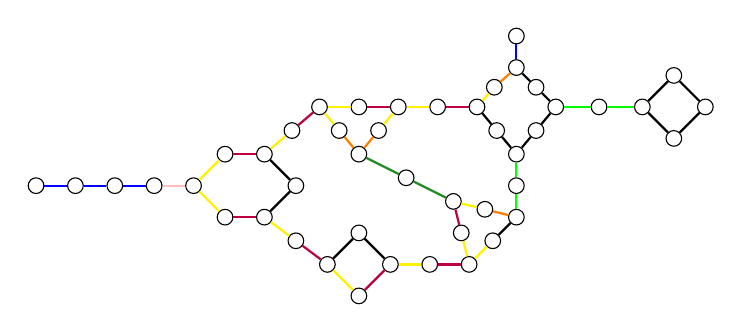
\begin{tikzpicture}
        \node[circle,draw,inner sep=2pt] (v00) at (-0.2,0.6) {};
        \node[circle,draw,inner sep=2pt] (v01) at (-0.2,1.4) {};
        \node[circle,draw,inner sep=2pt] (v02) at (-0.7,1.4) {};
        \node[circle,draw,inner sep=2pt] (v03) at (0.2,1) {};
        \node[circle,draw,inner sep=2pt] (v04) at (-0.7,0.6) {};
        \node[circle,draw,inner sep=2pt] (v05) at (-1.1,1) {};

        \node[circle,draw,inner sep=2pt] (s) at (-1.6,1) {};
        \node[circle,draw,inner sep=2pt] (n1) at (-2.1,1) {};
        \node[circle,draw,inner sep=2pt] (n2) at (-2.6,1) {};
        \node[circle,draw,inner sep=2pt] (n3) at (-3.1,1) {};

        \node[circle,draw,inner sep=2pt] (c01) at (0.15,1.7) {};

        \node[circle,draw,inner sep=2pt] (v10) at (0.5,2) {};
        \node[circle,draw,inner sep=2pt] (v11) at (1,1.4) {};
        \node[circle,draw,inner sep=2pt] (v12) at (1.5,2) {};
        \node[circle,draw,inner sep=2pt] (v13) at (0.75,1.7) {};
        \node[circle,draw,inner sep=2pt] (v14) at (1.25,1.7) {};
        \node[circle,draw,inner sep=2pt] (v15) at (1,2) {};

        \node[circle,draw,inner sep=2pt] (c02) at (0.2,0.3) {};

        \node[circle,draw,inner sep=2pt] (v20) at (0.6,0) {};
        \node[circle,draw,inner sep=2pt] (v21) at (1.4,0) {};
        \node[circle,draw,inner sep=2pt] (v22) at (1,-0.4) {};
        \node[circle,draw,inner sep=2pt] (v23) at (1,0.4) {};

        \node[circle,draw,inner sep=2pt] (c13) at (2,2) {};

        \node[circle,draw,inner sep=2pt] (v30) at (2.5,2) {};
        \node[circle,draw,inner sep=2pt] (v31) at (3,1.4) {};
        \node[circle,draw,inner sep=2pt] (v32) at (3.5,2) {};
        \node[circle,draw,inner sep=2pt] (v33) at (2.75,1.7) {};
        \node[circle,draw,inner sep=2pt] (v34) at (3.25,1.7) {};
        \node[circle,draw,inner sep=2pt] (v35) at (3.25,2.25) {};
        \node[circle,draw,inner sep=2pt] (v36) at (3,2.5) {};
        \node[circle,draw,inner sep=2pt] (v37) at (2.72,2.25) {};

        \node[circle,draw,inner sep=2pt] (g) at (3,2.9) {};

        \node[circle,draw,inner sep=2pt] (c14) at (1.6,1.1) {};
        \node[circle,draw,inner sep=2pt] (c24) at (1.9,0) {};
        \node[circle,draw,inner sep=2pt] (c34) at (3,1) {};
    
        \node[circle,draw,inner sep=2pt] (v40) at (2.4,0) {};
        \node[circle,draw,inner sep=2pt] (v41) at (2.2,0.8) {};
        \node[circle,draw,inner sep=2pt] (v42) at (3,0.6) {};
        \node[circle,draw,inner sep=2pt] (v43) at (2.3,0.4) {};
        \node[circle,draw,inner sep=2pt] (v44) at (2.6,0.7) {};
        \node[circle,draw,inner sep=2pt] (v45) at (2.7,0.3) {};
        
        \node[circle,draw,inner sep=2pt] (c35) at (4.05,2) {};

        \node[circle,draw,inner sep=2pt] (v50) at (5,1.6) {};
        \node[circle,draw,inner sep=2pt] (v51) at (5,2.4) {};
        \node[circle,draw,inner sep=2pt] (v52) at (4.6,2) {};
        \node[circle,draw,inner sep=2pt] (v53) at (5.4,2) {};

        \draw[thick,pink] (s) to (v05);
        \draw[thick,blue] (n1) to (s);
        \draw[thick,blue] (n2) to (n1);
        \draw[thick,blue] (n2) to (n3);

        \draw[thick,purple] (v00) to (v04);
        \draw[thick,yellow] (v05) to (v04);
        \draw[thick,yellow] (v02) to (v05);
        \draw[thick,purple] (v02) to (v01);
        \draw[thick] (v01) to (v03);
        \draw[thick] (v03) to (v00);

        \draw[thick,yellow] (v10) to (v13);
        \draw[thick,orange] (v13) to (v11);
        \draw[thick,orange] (v11) to (v14);
        \draw[thick,yellow] (v14) to (v12);
        \draw[thick,purple] (v12) to (v15);
        \draw[thick,yellow] (v15) to (v10);

        \draw[thick,yellow] (v20) to (v22);
        \draw[thick,purple] (v22) to (v21);
        \draw[thick] (v21) to (v23);
        \draw[thick] (v23) to (v20);

        \draw[thick] (v30) to (v33);
        \draw[thick] (v33) to (v31);
        \draw[thick] (v31) to (v34);
        \draw[thick] (v34) to (v32);
        \draw[thick] (v32) to (v35);
        \draw[thick] (v35) to (v36);
        \draw[thick,orange] (v36) to (v37);
        \draw[thick,yellow] (v37) to (v30);

        \draw[thick, blue] (v36) to (g);

        \draw[thick,yellow] (v40) to (v43);
        \draw[thick,purple] (v43) to (v41);
        \draw[thick,yellow] (v41) to (v44);
        \draw[thick,orange] (v44) to (v42);
        \draw[thick] (v42) to (v45);
        \draw[thick,yellow] (v45) to (v40);

        \draw[thick] (v50) to (v52);
        \draw[thick] (v52) to (v51);
        \draw[thick] (v51) to (v53);
        \draw[thick] (v53) to (v50);

        \draw[thick,yellow] (v00) -- (c02);
        \draw[thick,purple] (c02) -- (v20);

        \draw[thick,yellow] (v01) -- (c01);
        \draw[thick,purple] (c01) -- (v10);

        \draw[thick,yellow] (v12) -- (c13);
        \draw[thick,purple] (c13) -- (v30);

        \draw[thick,forestgreen] (v11) -- (c14);
        \draw[thick,forestgreen] (c14) -- (v41);

        \draw[thick,yellow] (v21) -- (c24);
        \draw[thick,purple] (c24) -- (v40);

        \draw[thick,green] (v31) -- (c34);
        \draw[thick,green] (c34) -- (v42);

        \draw[thick,green] (v32) -- (c35);
        \draw[thick,green] (c35) -- (v52);
    \end{tikzpicture}
\end{center}

In our example only one orange edge hits the blue goal edge, but in theory two orange edges could do that at the same time.
The following two rules detect that.

\begin{center}
    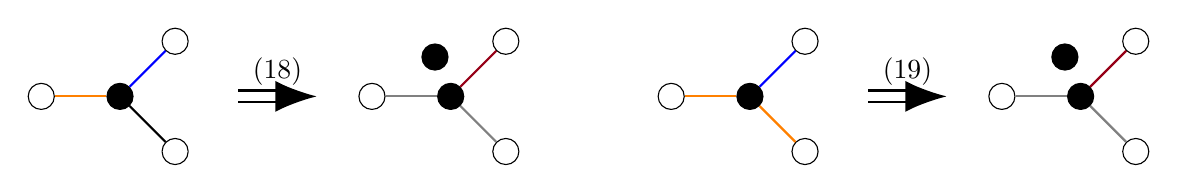
\begin{tikzpicture}
        % SplitRule(
        %     name="Discover goal (1)",
        %     input={"orange": 1, "black": 1, "blue": 1},
        %     node1_connection={"orange": "gray", "black": "gray", "blue": "crimson"},
        %     node2_connection={},
        % ),
        \begin{scope}[xshift=-4cm]
            \begin{scope}[xshift=-2cm]
                \node[circle,draw,fill] (A) at (0, 0) {};
                \node[circle,draw] (B) at (-1,0) {};
                \node[circle,draw] (C) at (0.7,0.7) {};
                \node[circle,draw] (D) at (0.7,-0.7) {};
                
                \draw[thick,orange] (A) -- (B);
                \draw[thick,blue] (A) -- (C);
                \draw[thick,black] (A) -- (D);
            \end{scope}
        
            \draw [line width=1pt, double distance=3pt, arrows = {-Latex[length=0pt 3 0]}] (-0.5,0) -- node[above] {(18)} (0.5,0);
            
            \begin{scope}[xshift=2.2cm]
                \node[circle,draw,fill] (A') at (-0.2, 0.5) {};
                \node[circle,draw,fill] (A) at (0, 0) {};
                \node[circle,draw] (B) at (-1,0) {};
                \node[circle,draw] (C) at (0.7,0.7) {};
                \node[circle,draw] (D) at (0.7,-0.7) {};
                
                \draw[thick,gray] (A) -- (B);
                \draw[thick,darkred] (A) -- (C);
                \draw[thick,gray] (A) -- (D);
            \end{scope}
        \end{scope}

        % SplitRule(
        %     name="Update next nodes (4)",
        %     input={"orange": 2, "lime": 1},
        %     node1_connection={"orange": "purple", "lime": "yellow"},
        %     node2_connection={},
        % ),
        \begin{scope}[xshift=4cm]
            \begin{scope}[xshift=-2cm]
                \node[circle,draw,fill] (A) at (0, 0) {};
                \node[circle,draw] (B) at (-1,0) {};
                \node[circle,draw] (C) at (0.7,0.7) {};
                \node[circle,draw] (D) at (0.7,-0.7) {};
                
                \draw[thick,orange] (A) -- (B);
                \draw[thick,blue] (A) -- (C);
                \draw[thick,orange] (A) -- (D);
            \end{scope}
        
            \draw [line width=1pt, double distance=3pt, arrows = {-Latex[length=0pt 3 0]}] (-0.5,0) -- node[above] {(19)} (0.5,0);
            
            \begin{scope}[xshift=2.2cm]
                \node[circle,draw,fill] (A') at (-0.2, 0.5) {};
                \node[circle,draw,fill] (A) at (0, 0) {};
                \node[circle,draw] (B) at (-1,0) {};
                \node[circle,draw] (C) at (0.7,0.7) {};
                \node[circle,draw] (D) at (0.7,-0.7) {};
                
                \draw[thick,gray] (A) -- (B);
                \draw[thick,darkred] (A) -- (C);
                \draw[thick,gray] (A) -- (D);
            \end{scope}
        \end{scope}
    \end{tikzpicture}
\end{center}

These edges turn the blue edge into a dark red one and change the neighboring edges to be gray.
This prepares the deletion of the entire graph so that only the counter remains.
This is done by a bunch of rules for deleting all nodes in the graph.

Let $S = \{yellow, orange, black, purple, green, dark green, olive\}$ be the colors that can appear in the graph.
For any $c_1 \in S$ and $c_2 \in S$ add the following rules.

\begin{center}
    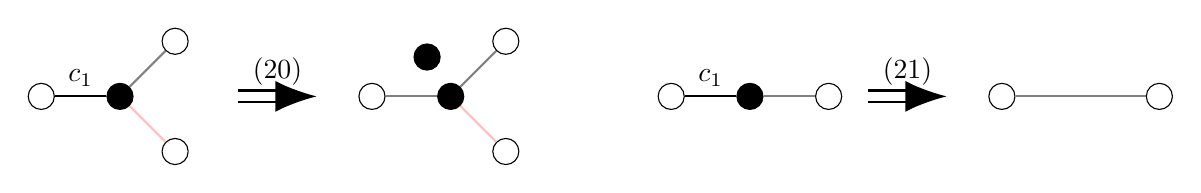
\begin{tikzpicture}
        % rules.append(SplitRule(
        %     name="Deletion at beginning (2)",
        %     input={c: 1, "gray": 1, "pink": 1},
        %     node1_connection={c: "gray", "gray": "gray", "pink": "pink"},
        %     node2_connection={},
        % ))
        \begin{scope}[xshift=-4cm]
            \begin{scope}[xshift=-2cm]
                \node[circle,draw,fill] (A) at (0, 0) {};
                \node[circle,draw] (B) at (-1,0) {};
                \node[circle,draw] (C) at (0.7,0.7) {};
                \node[circle,draw] (D) at (0.7,-0.7) {};
                
                \draw[thick] (A) -- node[above] {$c_1$} (B);
                \draw[thick,gray] (A) -- (C);
                \draw[thick,pink] (A) -- (D);
            \end{scope}
        
            \draw [line width=1pt, double distance=3pt, arrows = {-Latex[length=0pt 3 0]}] (-0.5,0) -- node[above] {(20)} (0.5,0);
            
            \begin{scope}[xshift=2.2cm]
                \node[circle,draw,fill] (A) at (0, 0) {};
                \node[circle,draw,fill] (A') at (-0.3, 0.5) {};
                \node[circle,draw] (B) at (-1,0) {};
                \node[circle,draw] (C) at (0.7,0.7) {};
                \node[circle,draw] (D) at (0.7,-0.7) {};
                
                \draw[thick,gray] (A) -- (B);
                \draw[thick,gray] (A) -- (C);
                \draw[thick,pink] (A) -- (D);
            \end{scope}
        \end{scope}

        % rules.append(DeleteRule(
        %     name="Delete color (1)",
        %     input={c: 1, "gray": 1},
        %     rewiring={(c, "gray"): "gray"},
        % ))
        \begin{scope}[xshift=4cm]
            \begin{scope}[xshift=-2cm]
                \node[circle,draw,fill] (A) at (0, 0) {};
                \node[circle,draw] (B) at (-1,0) {};
                \node[circle,draw] (C) at (1,0) {};
                
                \draw[thick] (A) -- node[above] {$c_1$} (B);
                \draw[thick,gray] (A) -- (C);
            \end{scope}
        
            \draw [line width=1pt, double distance=3pt, arrows = {-Latex[length=0pt 3 0]}] (-0.5,0) -- node[above] {(21)} (0.5,0);
            
            \begin{scope}[xshift=2.2cm]
                \node[circle,draw] (B) at (-1,0) {};
                \node[circle,draw] (C) at (1,0) {};
                
                \draw[thick,gray] (B) -- (C);
            \end{scope}
        \end{scope}
    \end{tikzpicture}

    \vspace*{0.5cm}

    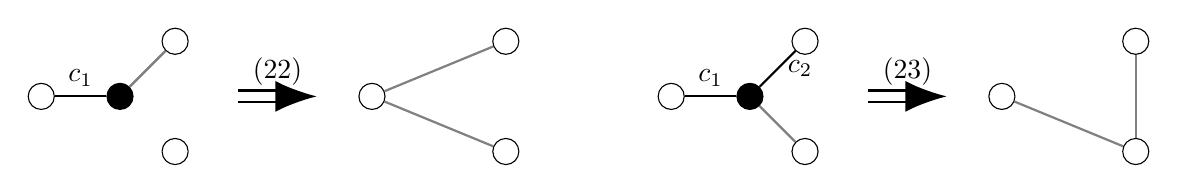
\begin{tikzpicture}
        % rules.append(DeleteRule(
        %     name="Delete color (2)",
        %     input={c: 1, "gray": 2},
        %     rewiring={(c, "gray"): "gray"},
        % ))
        \begin{scope}[xshift=-4cm]
            \begin{scope}[xshift=-2cm]
                \node[circle,draw,fill] (A) at (0, 0) {};
                \node[circle,draw] (B) at (-1,0) {};
                \node[circle,draw] (C) at (0.7,0.7) {};
                \node[circle,draw] (D) at (0.7,-0.7) {};
                
                \draw[thick] (A) -- node[above] {$c_1$} (B);
                \draw[thick,gray] (A) -- (C);
                \draw[thick,gray] (A) -- (C);
            \end{scope}
        
            \draw [line width=1pt, double distance=3pt, arrows = {-Latex[length=0pt 3 0]}] (-0.5,0) -- node[above] {(22)} (0.5,0);
            
            \begin{scope}[xshift=2.2cm]
                \node[circle,draw] (B) at (-1,0) {};
                \node[circle,draw] (C) at (0.7,0.7) {};
                \node[circle,draw] (D) at (0.7,-0.7) {};
                
                \draw[thick,gray] (B) -- (C);
                \draw[thick,gray] (B) -- (D);
            \end{scope}
        \end{scope}

        % for c2 in delete_colors[i+1:]:
        %     rules.append(DeleteRule(
        %         name="Delete color (4)",
        %         input={c1: 1, c2: 1, "gray": 1},
        %         rewiring={(c1, "gray"): "gray", (c2, "gray"): "gray"},
        %     ))
        \begin{scope}[xshift=4cm]
            \begin{scope}[xshift=-2cm]
                \node[circle,draw,fill] (A) at (0, 0) {};
                \node[circle,draw] (B) at (-1,0) {};
                \node[circle,draw] (C) at (0.7,0.7) {};
                \node[circle,draw] (D) at (0.7,-0.7) {};
                
                \draw[thick] (A) -- node[above] {$c_1$} (B);
                \draw[thick] (A) -- node[right] {$c_2$} (C);
                \draw[thick,gray] (A) -- (D);
            \end{scope}
        
            \draw [line width=1pt, double distance=3pt, arrows = {-Latex[length=0pt 3 0]}] (-0.5,0) -- node[above] {(23)} (0.5,0);
            
            \begin{scope}[xshift=2.2cm]
                \node[circle,draw] (B) at (-1,0) {};
                \node[circle,draw] (C) at (0.7,0.7) {};
                \node[circle,draw] (D) at (0.7,-0.7) {};
                
                \draw[thick,gray] (D) -- (C);
                \draw[thick,gray] (B) -- (D);
            \end{scope}
        \end{scope}
    \end{tikzpicture}
\end{center}

\begin{center}
    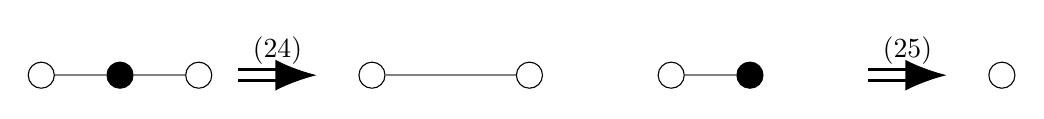
\begin{tikzpicture}
        % DeleteRule(
        %     name="Contract gray",
        %     input={"gray": 2},
        %     rewiring={("gray", "gray"): "gray"},
        % ),
        \begin{scope}[xshift=-4cm]
            \begin{scope}[xshift=-2cm]
                \node[circle,draw,fill] (A) at (0, 0) {};
                \node[circle,draw] (B) at (-1,0) {};
                \node[circle,draw] (C) at (1,0) {};
                
                \draw[thick,gray] (A) -- (B);
                \draw[thick,gray] (A) -- (C);
            \end{scope}
        
            \draw [line width=1pt, double distance=3pt, arrows = {-Latex[length=0pt 3 0]}] (-0.5,0) -- node[above] {(24)} (0.5,0);
            
            \begin{scope}[xshift=2.2cm]
                \node[circle,draw] (B) at (-1,0) {};
                \node[circle,draw] (C) at (1,0) {};
                
                \draw[thick,gray] (B) -- (C);
            \end{scope}
        \end{scope}

        % DeleteRule(
        %     name="Delete gray",
        %     input={"gray": 1},
        %     rewiring={},
        % ),
        \begin{scope}[xshift=4cm]
            \begin{scope}[xshift=-2cm]
                \node[circle,draw,fill] (A) at (0, 0) {};
                \node[circle,draw] (B) at (-1,0) {};
                
                \draw[thick,gray] (A) -- (B);
            \end{scope}
        
            \draw [line width=1pt, double distance=3pt, arrows = {-Latex[length=0pt 3 0]}] (-0.5,0) -- node[above] {(25)} (0.5,0);
            
            \begin{scope}[xshift=2.2cm]
                \node[circle,draw] (B) at (-1,0) {};
            \end{scope}
        \end{scope}
    \end{tikzpicture}

    \vspace*{0.5cm}

    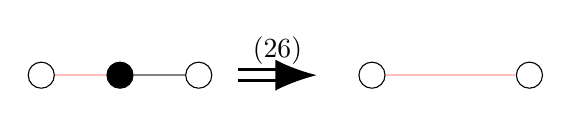
\begin{tikzpicture}
        % DeleteRule(
        %     name="Contract pink",
        %     input={"pink": 1, "gray": 1},
        %     rewiring={("pink", "gray"): "pink"},
        % ),
        \begin{scope}[xshift=-4cm]
            \begin{scope}[xshift=-2cm]
                \node[circle,draw,fill] (A) at (0, 0) {};
                \node[circle,draw] (B) at (-1,0) {};
                \node[circle,draw] (C) at (1,0) {};
                
                \draw[thick,pink] (A) -- (B);
                \draw[thick,gray] (A) -- (C);
            \end{scope}
        
            \draw [line width=1pt, double distance=3pt, arrows = {-Latex[length=0pt 3 0]}] (-0.5,0) -- node[above] {(26)} (0.5,0);
            
            \begin{scope}[xshift=2.2cm]
                \node[circle,draw] (B) at (-1,0) {};
                \node[circle,draw] (C) at (1,0) {};
                
                \draw[thick,pink] (B) -- (C);
            \end{scope}
        \end{scope}
    \end{tikzpicture}
\end{center}

These rules "spread out" the gray edges and delete the entire graph with this.
With these rules we also never cut the graph in half and the dark red edge will move closer to the pink one.
After the deletion is done the graph will look as follows.

\begin{center}
    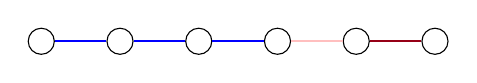
\begin{tikzpicture}
        \node[circle,draw] (v6) at (-1,0) {};
        \node[circle,draw] (v0) at (0,0) {};
        \node[circle,draw] (v1) at (1,0) {};
        \node[circle,draw] (v2) at (2,0) {};
        \node[circle,draw] (v3) at (3,0) {};
        \node[circle,draw] (v4) at (4,0) {};

        \draw[thick,blue] (v6) -- (v0);
        \draw[thick,blue] (v0) -- (v1);
        \draw[thick,blue] (v1) -- (v2);
        \draw[thick,pink] (v2) -- (v3);
        \draw[thick,darkred] (v3) -- (v4);
    \end{tikzpicture}
\end{center}

Two more rules detect that everthing was deleted and decrease the counter by one (since the counter was always one more than the distance we had explored).

\begin{center}
    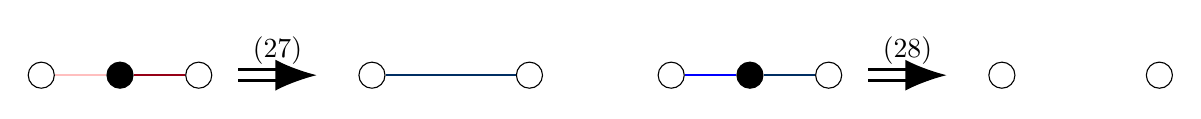
\begin{tikzpicture}
        % DeleteRule(
        %     name="Deleted everything",
        %     input={"pink": 1, "crimson": 1},
        %     rewiring={(("pink", "crimson")): "darkblue"},
        % ),
        \begin{scope}[xshift=-4cm]
            \begin{scope}[xshift=-2cm]
                \node[circle,draw,fill] (A) at (0, 0) {};
                \node[circle,draw] (B) at (-1,0) {};
                \node[circle,draw] (C) at (1,0) {};
                
                \draw[thick,pink] (A) -- (B);
                \draw[thick,darkred] (A) -- (C);
            \end{scope}
        
            \draw [line width=1pt, double distance=3pt, arrows = {-Latex[length=0pt 3 0]}] (-0.5,0) -- node[above] {(27)} (0.5,0);
            
            \begin{scope}[xshift=2.2cm]
                \node[circle,draw] (B) at (-1,0) {};
                \node[circle,draw] (C) at (1,0) {};
                
                \draw[thick,darkblue] (B) -- (C);
            \end{scope}
        \end{scope}

        % DeleteRule(
        %     name="Complete calculation",
        %     input={"darkblue": 1, "blue": 1},
        %     rewiring={},
        % ),
        \begin{scope}[xshift=4cm]
            \begin{scope}[xshift=-2cm]
                \node[circle,draw,fill] (A) at (0, 0) {};
                \node[circle,draw] (B) at (-1,0) {};
                \node[circle,draw] (C) at (1,0) {};
                
                \draw[thick,blue] (A) -- (B);
                \draw[thick,darkblue] (A) -- (C);
            \end{scope}
        
            \draw [line width=1pt, double distance=3pt, arrows = {-Latex[length=0pt 3 0]}] (-0.5,0) -- node[above] {(28)} (0.5,0);
            
            \begin{scope}[xshift=2.2cm]
                \node[circle,draw] (B) at (-1,0) {};
                \node[circle,draw] (C) at (1,0) {};
            \end{scope}
        \end{scope}
    \end{tikzpicture}
\end{center}

This results in the following final graph which is the correct result.

\begin{center}
    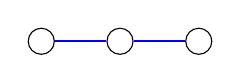
\begin{tikzpicture}
        \node[circle,draw] (v6) at (-1,0) {};
        \node[circle,draw] (v0) at (0,0) {};
        \node[circle,draw] (v1) at (1,0) {};

        \draw[thick,blue] (v6) -- (v0);
        \draw[thick,blue] (v0) -- (v1);
    \end{tikzpicture}
\end{center}

There are some scenarios which didn't happen in the example but need to be handle to make sure our algorithm works in the general case.
There are some special rules for handling vertices that had degree 1 in the original graph which are rather uninterresting.
Refer to the GitHub repository to find them.
Moreover, it can happen that we explore a green edge from both sides at the same time.
Then we will delete that edge to avoid other issues.

\begin{center}
    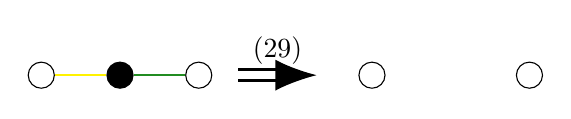
\begin{tikzpicture}
        % DeleteRule(
        %         name="Propagate update (node already reachable)",
        %         input={"yellow": 1, "lime": 1},
        %         rewiring={},
        %     ),
        \begin{scope}[xshift=-4cm]
            \begin{scope}[xshift=-2cm]
                \node[circle,draw,fill] (A) at (0, 0) {};
                \node[circle,draw] (B) at (-1,0) {};
                \node[circle,draw] (C) at (1,0) {};
                
                \draw[thick,yellow] (A) -- (B);
                \draw[thick,forestgreen] (A) -- (C);
            \end{scope}
        
            \draw [line width=1pt, double distance=3pt, arrows = {-Latex[length=0pt 3 0]}] (-0.5,0) -- node[above] {(29)} (0.5,0);
            
            \begin{scope}[xshift=2.2cm]
                \node[circle,draw] (B) at (-1,0) {};
                \node[circle,draw] (C) at (1,0) {};
            \end{scope}
        \end{scope}
    \end{tikzpicture}
\end{center}

This complete my more complex example of determining the length of the shortest paths between two vertices in a graph.


\section{Reduction to Turing Machines}

In this section, I will reduce a Turing Machine $\langle Q, \Sigma, \Gamma, \delta, q_0, q_{halt} \rangle$ to a Colored Graph.
Instead of using actual colors, the set of colors will also contain elements like the states of the Turing Machine.
This makes it clearer which part of the Turing machine is represented by which part of the Colored Graph.
For our Colored Graph we will use the colors $\C = Q \cup \Gamma \cup \{L, R, L', R', end, end_2, end_3\}$.
I will write the name of the color next to the edges.

First, we need to encode the state of the Turing Machine.
Let $\ldots\sqcup\sqcup x_1 x_2 \ldots x_{i-1} x_{i} x_{i+1} \ldots x_k \sqcup\sqcup\ldots$ be the tape content of the Turing Machine with the head of the Turing machine pointed at $x_i$ and $q$ the current state.
Then we construct the Colored Graph as follows.

\begin{center}
    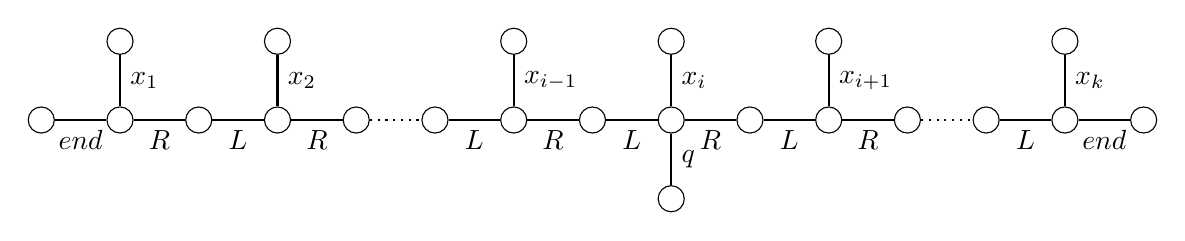
\begin{tikzpicture}
        \node[circle,draw] (A) at (1,0) {};
        \node[circle,draw] (B) at (2,0) {};
        \node[circle,draw] (Bs) at (2,1) {};
        \node[circle,draw] (C) at (3,0) {};
        \node[circle,draw] (D) at (4,0) {};
        \node[circle,draw] (Ds) at (4,1) {};
        \node[circle,draw] (E) at (5,0) {};
        \node[circle,draw] (F) at (6,0) {};
        \node[circle,draw] (G) at (7,0) {};
        \node[circle,draw] (Gs) at (7,1) {};
        \node[circle,draw] (H) at (8,0) {};
        \node[circle,draw] (I) at (9,0) {};
        \node[circle,draw] (Is) at (9,1) {};
        \node[circle,draw] (J) at (10,0) {};
        \node[circle,draw] (K) at (11,0) {};
        \node[circle,draw] (Ks) at (11,1) {};
        \node[circle,draw] (L) at (12,0) {};
        \node[circle,draw] (M) at (13,0) {};
        \node[circle,draw] (N) at (14,0) {};
        \node[circle,draw] (Ns) at (14,1) {};
        \node[circle,draw] (O) at (15,0) {};
        
        \node[circle,draw] (S) at (9,-1) {};
        \draw[thick] (S) -- node[right] {$q$} (I);
        
        \draw[thick] (A) -- node[below] {$end$} (B);
        \draw[thick] (B) -- node[right] {$x_1$} (Bs);
        \draw[thick] (B) -- node[below] {$R$} (C);
        \draw[thick] (C) -- node[below] {$L$} (D);
        \draw[thick] (D) -- node[right] {$x_2$} (Ds);
        \draw[thick] (D) -- node[below] {$R$} (E);
        \draw[thick, dotted] (E) -- node[below] {} (F);
        \draw[thick] (F) -- node[below] {$L$} (G);
        \draw[thick] (G) -- node[below] {$R$} (H);
        \draw[thick] (G) -- node[right] {$x_{i-1}$} (Gs);
        \draw[thick] (H) -- node[below] {$L$} (I);
        \draw[thick] (I) -- node[right] {$x_i$} (Is);
        \draw[thick] (I) -- node[below] {$R$} (J);
        \draw[thick] (J) -- node[below] {$L$} (K);
        \draw[thick] (K) -- node[right] {$x_{i+1}$} (Ks);
        \draw[thick] (K) -- node[below] {$R$} (L);
        \draw[thick, dotted] (L) -- node[below] {} (M);
        \draw[thick] (M) -- node[below] {$L$} (N);
        \draw[thick] (N) -- node[right] {$x_k$} (Ns);
        \draw[thick] (N) -- node[below] {$end$} (O);
    \end{tikzpicture}
\end{center}

To avoid handling multiple special cases we will also make sure that the Colored Graph always has at least two cells of the Turing machine.
So even for an empty tape we have two cells that are simply marked with the placeholder symbol $\sqcup$.

The rules to emulate the Turing Machine are as follows.

\begin{itemize}
    \item For each transition $\delta(q, x) = (q', y, R)$ we add the following rule.
    \begin{center}
        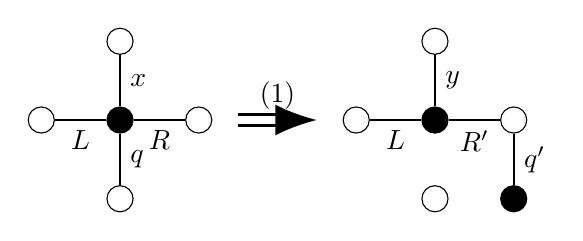
\begin{tikzpicture}
        \begin{scope}[xshift=-2cm]
            \node[circle,draw,fill] (A) at (0, 0) {};
            \node[circle,draw] (B) at (-1,0) {};
            \node[circle,draw] (C) at (0,1) {};
            \node[circle,draw] (D) at (1,0) {};
            \node[circle,draw] (E) at (0,-1) {};
            
            \draw[thick] (A) -- node[below] {$L$} (B);
            \draw[thick] (A) -- node[right] {$x$} (C);
            \draw[thick] (A) -- node[below] {$R$} (D);
            \draw[thick] (A) -- node[right] {$q$} (E);
        \end{scope}
    
        \draw [line width=1pt, double distance=3pt, arrows = {-Latex[length=0pt 3 0]}] (-0.5,0) -- node[above] {(1)} (0.5,0);
        
        \begin{scope}[xshift=2cm]
            \node[circle,draw,fill] (A) at (0, 0) {};
            \node[circle,draw,fill] (A') at (1, -1) {};
            \node[circle,draw] (B) at (-1,0) {};
            \node[circle,draw] (C) at (0,1) {};
            \node[circle,draw] (D) at (1,0) {};
            \node[circle,draw] (E) at (0,-1) {};

            \draw[thick] (A) -- node[below] {$L$} (B);
            \draw[thick] (A) -- node[right] {$y$} (C);
            \draw[thick] (A) -- node[below] {$R'$} (D);
            \draw[thick] (A') -- node[right] {$q'$} (D);
        \end{scope}
        \end{tikzpicture}
    \end{center}
    \item For each transition $\delta(q, x) = (q', y, L)$ we add the following rule.
    \begin{center}
        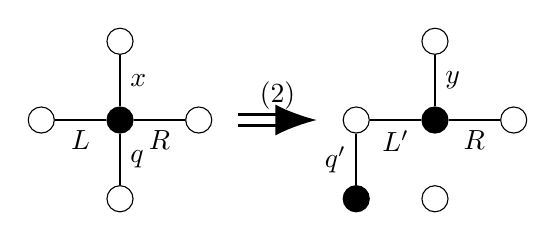
\begin{tikzpicture}
        \begin{scope}[xshift=-2cm]
            \node[circle,draw,fill] (A) at (0, 0) {};
            \node[circle,draw] (B) at (-1,0) {};
            \node[circle,draw] (C) at (0,1) {};
            \node[circle,draw] (D) at (1,0) {};
            \node[circle,draw] (E) at (0,-1) {};
            
            \draw[thick] (A) -- node[below] {$L$} (B);
            \draw[thick] (A) -- node[right] {$x$} (C);
            \draw[thick] (A) -- node[below] {$R$} (D);
            \draw[thick] (A) -- node[right] {$q$} (E);
        \end{scope}
    
        \draw [line width=1pt, double distance=3pt, arrows = {-Latex[length=0pt 3 0]}] (-0.5,0) -- node[above] {(2)} (0.5,0);
        
        \begin{scope}[xshift=2cm]
            \node[circle,draw,fill] (A) at (0, 0) {};
            \node[circle,draw,fill] (A') at (-1, -1) {};
            \node[circle,draw] (B) at (-1,0) {};
            \node[circle,draw] (C) at (0,1) {};
            \node[circle,draw] (D) at (1,0) {};
            \node[circle,draw] (E) at (0,-1) {};

            \draw[thick] (A) -- node[below] {$L'$} (B);
            \draw[thick] (A) -- node[right] {$y$} (C);
            \draw[thick] (A) -- node[below] {$R$} (D);
            \draw[thick] (A') -- node[left] {$q'$} (B);
        \end{scope}
        \end{tikzpicture}
    \end{center}
    \item Next for each $q \in Q$ we add the following two rules.
    \begin{center}
        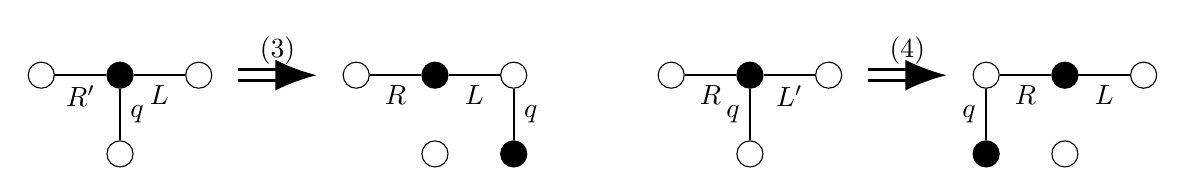
\begin{tikzpicture}
        \begin{scope}[xshift=-4cm]
            \begin{scope}[xshift=-2cm]
                \node[circle,draw,fill] (A) at (0, 0) {};
                \node[circle,draw] (B) at (-1,0) {};
                \node[circle,draw] (D) at (1,0) {};
                \node[circle,draw] (E) at (0,-1) {};
                
                \draw[thick] (A) -- node[below] {$R'$} (B);
                \draw[thick] (A) -- node[below] {$L$} (D);
                \draw[thick] (A) -- node[right] {$q$} (E);
            \end{scope}
        
            \draw [line width=1pt, double distance=3pt, arrows = {-Latex[length=0pt 3 0]}] (-0.5,0) -- node[above] {(3)} (0.5,0);
            
            \begin{scope}[xshift=2cm]
                \node[circle,draw,fill] (A) at (0, 0) {};
                \node[circle,draw,fill] (A') at (1, -1) {};
                \node[circle,draw] (B) at (-1,0) {};
                \node[circle,draw] (D) at (1,0) {};
                \node[circle,draw] (E) at (0,-1) {};
    
                \draw[thick] (A) -- node[below] {$R$} (B);
                \draw[thick] (A) -- node[below] {$L$} (D);
                \draw[thick] (A') -- node[right] {$q$} (D);
            \end{scope}
        \end{scope}

        \begin{scope}[xshift=4cm]
            \begin{scope}[xshift=-2cm]
                \node[circle,draw,fill] (A) at (0, 0) {};
                \node[circle,draw] (B) at (-1,0) {};
                \node[circle,draw] (D) at (1,0) {};
                \node[circle,draw] (E) at (0,-1) {};
                
                \draw[thick] (A) -- node[below] {$R$} (B);
                \draw[thick] (A) -- node[below] {$L'$} (D);
                \draw[thick] (A) -- node[left] {$q$} (E);
            \end{scope}
        
            \draw [line width=1pt, double distance=3pt, arrows = {-Latex[length=0pt 3 0]}] (-0.5,0) -- node[above] {(4)} (0.5,0);
            
            \begin{scope}[xshift=2cm]
                \node[circle,draw,fill] (A) at (0, 0) {};
                \node[circle,draw,fill] (A') at (-1, -1) {};
                \node[circle,draw] (B) at (-1,0) {};
                \node[circle,draw] (D) at (1,0) {};
                \node[circle,draw] (E) at (0,-1) {};
    
                \draw[thick] (A) -- node[below] {$R$} (B);
                \draw[thick] (A) -- node[below] {$L$} (D);
                \draw[thick] (A') -- node[left] {$q$} (B);
            \end{scope}
        \end{scope}
        \end{tikzpicture}
    \end{center}
    \item Since we create isolated vertices with some rules, we add a Delete Rule that just deletes such vertices.
    \begin{center}
        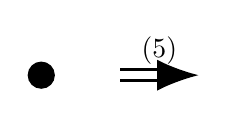
\begin{tikzpicture}
        \begin{scope}[xshift=-1.5cm]
            \node[circle,draw,fill] (A) at (0, 0) {};
        \end{scope}
    
        \draw [line width=1pt, double distance=3pt, arrows = {-Latex[length=0pt 3 0]}] (-0.5,0) -- node[above] {(5)} (0.5,0);
        
        \begin{scope}[xshift=2cm]
        \end{scope}
        \end{tikzpicture}
    \end{center}
\end{itemize}

There are still 6 rules missing to deal with the edge of the tape, but these rules alone can simulate a transition of the Turing machine.
So before introducing the remaining rules let's first see an example transition.
For this we will only look at the relavent section of the Turing machine where the head is currently pointing to.
Assume we have a transition $\delta(q, x) = (q', y, R)$.
Then the Colored graph will evolve as follows where I will always mark the node a rule will be applied to in the next step with black.

\begin{center}
    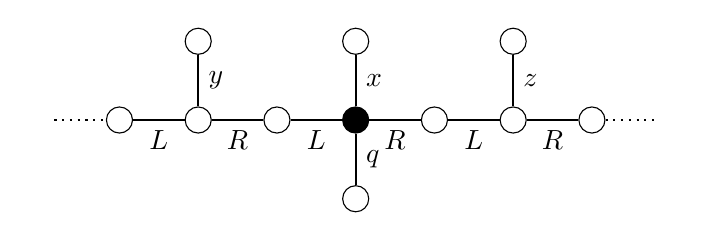
\begin{tikzpicture}
        \node[circle] (E) at (5,0) {};
        \node[circle,draw] (F) at (6,0) {};
        \node[circle,draw] (G) at (7,0) {};
        \node[circle,draw] (Gs) at (7,1) {};
        \node[circle,draw] (H) at (8,0) {};
        \node[circle,draw,fill] (I) at (9,0) {};
        \node[circle,draw] (Is) at (9,1) {};
        \node[circle,draw] (J) at (10,0) {};
        \node[circle,draw] (K) at (11,0) {};
        \node[circle,draw] (Ks) at (11,1) {};
        \node[circle,draw] (L) at (12,0) {};
        \node[circle] (M) at (13,0) {};
        
        \node[circle,draw] (S) at (9,-1) {};
        \draw[thick] (S) -- node[right] {$q$} (I);
        
        \draw[thick, dotted] (E) -- node[below] {} (F);
        \draw[thick] (F) -- node[below] {$L$} (G);
        \draw[thick] (G) -- node[right] {$y$} (Gs);
        \draw[thick] (G) -- node[below] {$R$} (H);
        \draw[thick] (H) -- node[below] {$L$} (I);
        \draw[thick] (I) -- node[right] {$x$} (Is);
        \draw[thick] (I) -- node[below] {$R$} (J);
        \draw[thick] (J) -- node[below] {$L$} (K);
        \draw[thick] (K) -- node[right] {$z$} (Ks);
        \draw[thick] (K) -- node[below] {$R$} (L);
        \draw[thick, dotted] (L) -- node[below] {} (M);
    \end{tikzpicture}
\end{center}

First, the node the head is pointing to is the only node that a rule can be applied to so rule (1) will be applied to it.

\begin{center}
    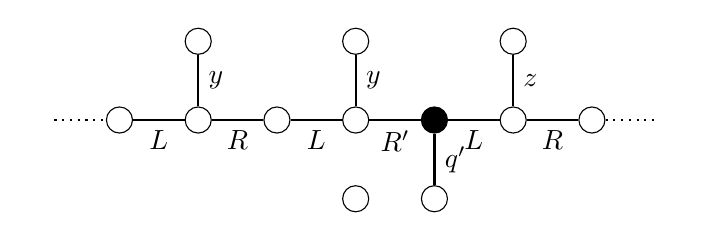
\begin{tikzpicture}
        \node[circle] (E) at (5,0) {};
        \node[circle,draw] (F) at (6,0) {};
        \node[circle,draw] (G) at (7,0) {};
        \node[circle,draw] (Gs) at (7,1) {};
        \node[circle,draw] (H) at (8,0) {};
        \node[circle,draw] (I) at (9,0) {};
        \node[circle,draw] (Is) at (9,1) {};
        \node[circle,draw,fill] (J) at (10,0) {};
        \node[circle,draw] (K) at (11,0) {};
        \node[circle,draw] (Ks) at (11,1) {};
        \node[circle,draw] (L) at (12,0) {};
        \node[circle] (M) at (13,0) {};
        
        \node[circle,draw] (S') at (9,-1) {};
        \node[circle,draw] (S) at (10,-1) {};
        \draw[thick] (S) -- node[right] {$q'$} (J);
        
        \draw[thick, dotted] (E) -- node[below] {} (F);
        \draw[thick] (F) -- node[below] {$L$} (G);
        \draw[thick] (G) -- node[right] {$y$} (Gs);
        \draw[thick] (G) -- node[below] {$R$} (H);
        \draw[thick] (H) -- node[below] {$L$} (I);
        \draw[thick] (I) -- node[right] {$y$} (Is);
        \draw[thick] (I) -- node[below] {$R'$} (J);
        \draw[thick] (J) -- node[below] {$L$} (K);
        \draw[thick] (K) -- node[right] {$z$} (Ks);
        \draw[thick] (K) -- node[below] {$R$} (L);
        \draw[thick, dotted] (L) -- node[below] {} (M);
    \end{tikzpicture}
\end{center}

Now we can either apply rule (5) to the isolated vertex or rule (3) to the node marked in black.
Since these nodes are disconnected it is clear that the order of application does not matter.
Here, we will apply rule (3) first resulting in the following.

\begin{center}
    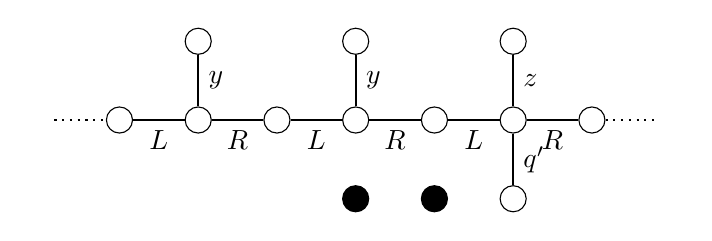
\begin{tikzpicture}
        \node[circle] (E) at (5,0) {};
        \node[circle,draw] (F) at (6,0) {};
        \node[circle,draw] (G) at (7,0) {};
        \node[circle,draw] (Gs) at (7,1) {};
        \node[circle,draw] (H) at (8,0) {};
        \node[circle,draw] (I) at (9,0) {};
        \node[circle,draw] (Is) at (9,1) {};
        \node[circle,draw] (J) at (10,0) {};
        \node[circle,draw] (K) at (11,0) {};
        \node[circle,draw] (Ks) at (11,1) {};
        \node[circle,draw] (L) at (12,0) {};
        \node[circle] (M) at (13,0) {};
        
        \node[circle,draw,fill] (S') at (9,-1) {};
        \node[circle,draw,fill] (S'') at (10,-1) {};
        \node[circle,draw] (S) at (11,-1) {};
        \draw[thick] (S) -- node[right] {$q'$} (K);
        
        \draw[thick, dotted] (E) -- node[below] {} (F);
        \draw[thick] (F) -- node[below] {$L$} (G);
        \draw[thick] (G) -- node[right] {$y$} (Gs);
        \draw[thick] (G) -- node[below] {$R$} (H);
        \draw[thick] (H) -- node[below] {$L$} (I);
        \draw[thick] (I) -- node[right] {$y$} (Is);
        \draw[thick] (I) -- node[below] {$R$} (J);
        \draw[thick] (J) -- node[below] {$L$} (K);
        \draw[thick] (K) -- node[right] {$z$} (Ks);
        \draw[thick] (K) -- node[below] {$R$} (L);
        \draw[thick, dotted] (L) -- node[below] {} (M);
    \end{tikzpicture}
\end{center}

With two applications of rule (5) we can delete the isolated vertices and complete the Turing machine transition.
Of course the rules for the next transition could also already be applied but the isolated will be deleted eventually as long as the Turing machine terminates and otherwise thay have no influence on the the rest of the graph.

\begin{center}
    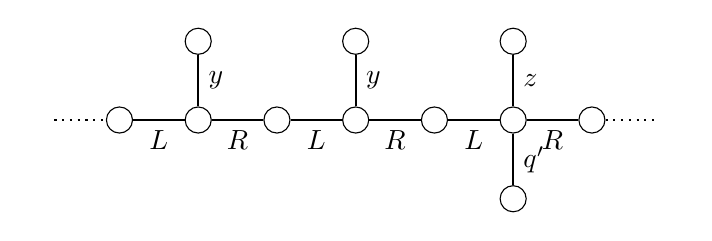
\begin{tikzpicture}
        \node[circle] (E) at (5,0) {};
        \node[circle,draw] (F) at (6,0) {};
        \node[circle,draw] (G) at (7,0) {};
        \node[circle,draw] (Gs) at (7,1) {};
        \node[circle,draw] (H) at (8,0) {};
        \node[circle,draw] (I) at (9,0) {};
        \node[circle,draw] (Is) at (9,1) {};
        \node[circle,draw] (J) at (10,0) {};
        \node[circle,draw] (K) at (11,0) {};
        \node[circle,draw] (Ks) at (11,1) {};
        \node[circle,draw] (L) at (12,0) {};
        \node[circle] (M) at (13,0) {};

        \node[circle,draw] (S) at (11,-1) {};
        \draw[thick] (S) -- node[right] {$q'$} (K);
        
        \draw[thick, dotted] (E) -- node[below] {} (F);
        \draw[thick] (F) -- node[below] {$L$} (G);
        \draw[thick] (G) -- node[right] {$y$} (Gs);
        \draw[thick] (G) -- node[below] {$R$} (H);
        \draw[thick] (H) -- node[below] {$L$} (I);
        \draw[thick] (I) -- node[right] {$y$} (Is);
        \draw[thick] (I) -- node[below] {$R$} (J);
        \draw[thick] (J) -- node[below] {$L$} (K);
        \draw[thick] (K) -- node[right] {$z$} (Ks);
        \draw[thick] (K) -- node[below] {$R$} (L);
        \draw[thick, dotted] (L) -- node[below] {} (M);
    \end{tikzpicture}
\end{center}

A transition that moves the head to the left can similarly be simulated by rules (2) and (4).

What's left to perform a complete simulation of t Turing machine is handling the edges of the tape.
For this we will add rules that extend the tape once the head reaches them.
Note that it is important to only extend the tape once the head actually reaches them, otherwise they could be extended indefinetly and the reduction of the Colored graph would not terminate.
For each $x \in \Gamma$ and $q \in Q$ we add the following rules.

\begin{center}
    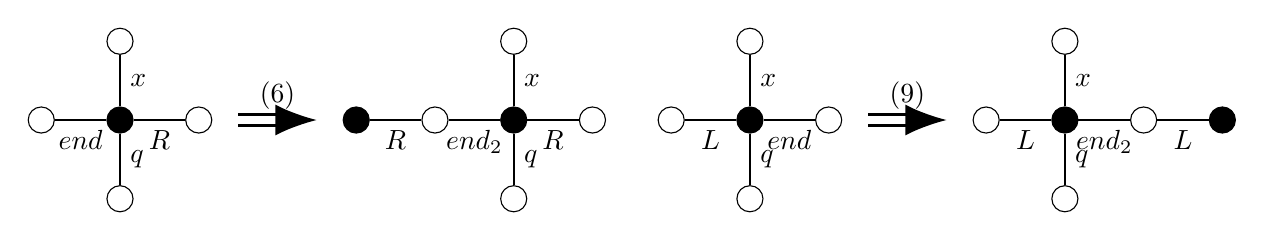
\begin{tikzpicture}
    \begin{scope}[xshift=-4cm]
        \begin{scope}[xshift=-2cm]
            \node[circle,draw,fill] (A) at (0, 0) {};
            \node[circle,draw] (B) at (-1,0) {};
            \node[circle,draw] (C) at (0,1) {};
            \node[circle,draw] (D) at (1,0) {};
            \node[circle,draw] (E) at (0,-1) {};
            
            \draw[thick] (A) -- node[right] {$x$} (C);
            \draw[thick] (A) -- node[right] {$q$} (E);
            \draw[thick] (A) -- node[below] {$end$} (B);
            \draw[thick] (A) -- node[below] {$R$} (D);
        \end{scope}
    
        \draw [line width=1pt, double distance=3pt, arrows = {-Latex[length=0pt 3 0]}] (-0.5,0) -- node[above] {(6)} (0.5,0);
        
        \begin{scope}[xshift=3cm]
            \node[circle,draw,fill] (A) at (0, 0) {};
            \node[circle,draw,fill] (A') at (-2, 0) {};
            \node[circle,draw] (B) at (-1,0) {};
            \node[circle,draw] (C) at (0,1) {};
            \node[circle,draw] (D) at (1,0) {};
            \node[circle,draw] (E) at (0,-1) {};
            
            \draw[thick] (A) -- node[right] {$x$} (C);
            \draw[thick] (A) -- node[right] {$q$} (E);
            \draw[thick] (A) -- node[below] {$end_2$} (B);
            \draw[thick] (A) -- node[below] {$R$} (D);
            \draw[thick] (A') -- node[below] {$R$} (B);
        \end{scope}
    \end{scope}

    \begin{scope}[xshift=4cm]
        \begin{scope}[xshift=-2cm]
            \node[circle,draw,fill] (A) at (0, 0) {};
            \node[circle,draw] (B) at (-1,0) {};
            \node[circle,draw] (C) at (0,1) {};
            \node[circle,draw] (D) at (1,0) {};
            \node[circle,draw] (E) at (0,-1) {};
            
            \draw[thick] (A) -- node[right] {$x$} (C);
            \draw[thick] (A) -- node[right] {$q$} (E);
            \draw[thick] (A) -- node[below] {$L$} (B);
            \draw[thick] (A) -- node[below] {$end$} (D);
        \end{scope}
    
        \draw [line width=1pt, double distance=3pt, arrows = {-Latex[length=0pt 3 0]}] (-0.5,0) -- node[above] {(9)} (0.5,0);
        
        \begin{scope}[xshift=2cm]
            \node[circle,draw,fill] (A) at (0, 0) {};
            \node[circle,draw,fill] (A') at (2, 0) {};
            \node[circle,draw] (B) at (-1,0) {};
            \node[circle,draw] (C) at (0,1) {};
            \node[circle,draw] (D) at (1,0) {};
            \node[circle,draw] (E) at (0,-1) {};
            
            \draw[thick] (A) -- node[right] {$x$} (C);
            \draw[thick] (A) -- node[right] {$q$} (E);
            \draw[thick] (A) -- node[below] {$L$} (B);
            \draw[thick] (A) -- node[below] {$end_2$} (D);
            \draw[thick] (A') -- node[below] {$L$} (D);
        \end{scope}
    \end{scope}
    \end{tikzpicture}

    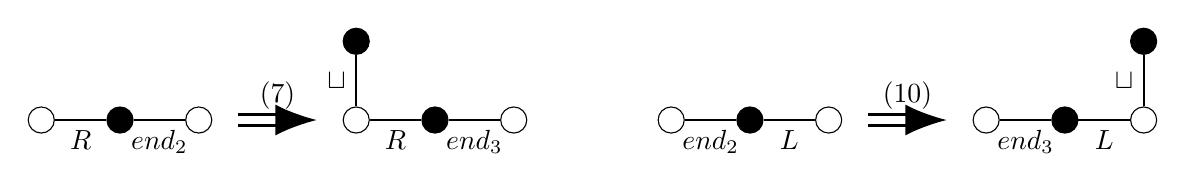
\begin{tikzpicture}
        \begin{scope}[xshift=-4cm]
            \begin{scope}[xshift=-2cm]
                \node[circle,draw,fill] (A) at (0, 0) {};
                \node[circle,draw] (B) at (-1,0) {};
                \node[circle,draw] (D) at (1,0) {};
                
                \draw[thick] (A) -- node[below] {$R$} (B);
                \draw[thick] (A) -- node[below] {$end_2$} (D);
            \end{scope}
        
            \draw [line width=1pt, double distance=3pt, arrows = {-Latex[length=0pt 3 0]}] (-0.5,0) -- node[above] {(7)} (0.5,0);
            
            \begin{scope}[xshift=2cm]
                \node[circle,draw,fill] (A) at (0, 0) {};
                \node[circle,draw,fill] (A') at (-1, 1) {};
                \node[circle,draw] (B) at (-1,0) {};
                \node[circle,draw] (D) at (1,0) {};
                
                \draw[thick] (A) -- node[below] {$R$} (B);
                \draw[thick] (A) -- node[below] {$end_3$} (D);
                \draw[thick] (A') -- node[left] {$\sqcup$} (B);
            \end{scope}
        \end{scope}

        \begin{scope}[xshift=4cm]
            \begin{scope}[xshift=-2cm]
                \node[circle,draw,fill] (A) at (0, 0) {};
                \node[circle,draw] (B) at (-1,0) {};
                \node[circle,draw] (D) at (1,0) {};
                
                \draw[thick] (A) -- node[below] {$end_2$} (B);
                \draw[thick] (A) -- node[below] {$L$} (D);
            \end{scope}
        
            \draw [line width=1pt, double distance=3pt, arrows = {-Latex[length=0pt 3 0]}] (-0.5,0) -- node[above] {(10)} (0.5,0);
            
            \begin{scope}[xshift=2cm]
                \node[circle,draw,fill] (A) at (0, 0) {};
                \node[circle,draw,fill] (A') at (1, 1) {};
                \node[circle,draw] (B) at (-1,0) {};
                \node[circle,draw] (D) at (1,0) {};
                
                \draw[thick] (A) -- node[below] {$end_3$} (B);
                \draw[thick] (A) -- node[below] {$L$} (D);
                \draw[thick] (A') -- node[left] {$\sqcup$} (D);
            \end{scope}
        \end{scope}
        \end{tikzpicture}

        \vspace*{0.8cm}

        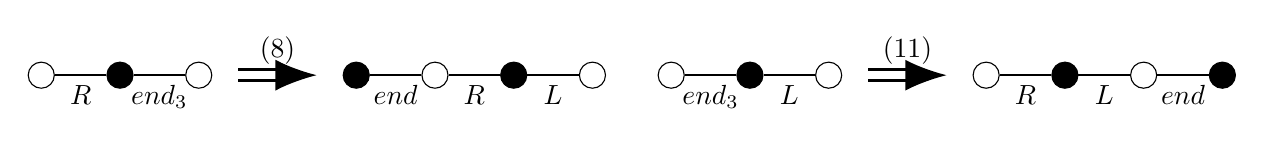
\begin{tikzpicture}
            \begin{scope}[xshift=-4cm]
                \begin{scope}[xshift=-2cm]
                    \node[circle,draw,fill] (A) at (0, 0) {};
                    \node[circle,draw] (B) at (-1,0) {};
                    \node[circle,draw] (D) at (1,0) {};
                    
                    \draw[thick] (A) -- node[below] {$R$} (B);
                    \draw[thick] (A) -- node[below] {$end_3$} (D);
                \end{scope}
            
                \draw [line width=1pt, double distance=3pt, arrows = {-Latex[length=0pt 3 0]}] (-0.5,0) -- node[above] {(8)} (0.5,0);
                
                \begin{scope}[xshift=3cm]
                    \node[circle,draw,fill] (A) at (0, 0) {};
                    \node[circle,draw,fill] (A') at (-2, 0) {};
                    \node[circle,draw] (B) at (-1,0) {};
                    \node[circle,draw] (D) at (1,0) {};
                    
                    \draw[thick] (A) -- node[below] {$R$} (B);
                    \draw[thick] (A) -- node[below] {$L$} (D);
                    \draw[thick] (A') -- node[below] {$end$} (B);
                \end{scope}
            \end{scope}
    
            \begin{scope}[xshift=4cm]
                \begin{scope}[xshift=-2cm]
                    \node[circle,draw,fill] (A) at (0, 0) {};
                    \node[circle,draw] (B) at (-1,0) {};
                    \node[circle,draw] (D) at (1,0) {};
                    
                    \draw[thick] (A) -- node[below] {$end_3$} (B);
                    \draw[thick] (A) -- node[below] {$L$} (D);
                \end{scope}
            
                \draw [line width=1pt, double distance=3pt, arrows = {-Latex[length=0pt 3 0]}] (-0.5,0) -- node[above] {(11)} (0.5,0);
                
                \begin{scope}[xshift=2cm]
                    \node[circle,draw,fill] (A) at (0, 0) {};
                    \node[circle,draw,fill] (A') at (2, 0) {};
                    \node[circle,draw] (B) at (-1,0) {};
                    \node[circle,draw] (D) at (1,0) {};
                    
                    \draw[thick] (A) -- node[below] {$R$} (B);
                    \draw[thick] (A) -- node[below] {$L$} (D);
                    \draw[thick] (A') -- node[below] {$end$} (D);
                \end{scope}
            \end{scope}
        \end{tikzpicture}
\end{center}

The extension of the tape will be handled in states as we need to add multiple nodes.
The stages are marked with the $end_i$ colors.
First when the head hits one of the tape borders, we add a new node to that side.
Then we add the placeholder $\sqcup$ to that new node.
Finally we add a new node that marks the new end of the tape.
An example entension of the left side of the tape would look at follows, where we apply rule (6), (7) and (8) in that order.

\begin{center}
    \begin{tikzpicture}
        \node[circle,draw] (A) at (1,0) {};
        \node[circle,draw,fill] (B) at (2,0) {};
        \node[circle,draw] (Bs) at (2,1) {};
        \node[circle,draw] (C) at (3,0) {};
        \node[circle,draw] (D) at (4,0) {};
        \node[circle,draw] (Ds) at (4,1) {};
        \node[circle,draw] (E) at (5,0) {};
        \node[circle] (F) at (6,0) {};
        
        \node[circle,draw] (S) at (2,-1) {};
        \draw[thick] (S) -- node[right] {$q$} (B);
        
        \draw[thick] (A) -- node[below] {$end$} (B);
        \draw[thick] (B) -- node[right] {$x$} (Bs);
        \draw[thick] (B) -- node[below] {$R$} (C);
        \draw[thick] (C) -- node[below] {$L$} (D);
        \draw[thick] (D) -- node[right] {$y$} (Ds);
        \draw[thick] (D) -- node[below] {$R$} (E);
        \draw[thick, dotted] (E) -- node[below] {} (F);
    \end{tikzpicture}
\end{center}

\begin{center}
    \begin{tikzpicture}
        \node[circle,draw] (N) at (0,0) {};
        \node[circle,draw,fill] (A) at (1,0) {};
        \node[circle,draw] (B) at (2,0) {};
        \node[circle,draw] (Bs) at (2,1) {};
        \node[circle,draw] (C) at (3,0) {};
        \node[circle,draw] (D) at (4,0) {};
        \node[circle,draw] (Ds) at (4,1) {};
        \node[circle,draw] (E) at (5,0) {};
        \node[circle] (F) at (6,0) {};
        
        \node[circle,draw] (S) at (2,-1) {};
        \draw[thick] (S) -- node[right] {$q$} (B);
        
        \draw[thick] (N) -- node[below] {$R$} (A);
        \draw[thick] (A) -- node[below] {$end_2$} (B);
        \draw[thick] (B) -- node[right] {$x$} (Bs);
        \draw[thick] (B) -- node[below] {$R$} (C);
        \draw[thick] (C) -- node[below] {$L$} (D);
        \draw[thick] (D) -- node[right] {$y$} (Ds);
        \draw[thick] (D) -- node[below] {$R$} (E);
        \draw[thick, dotted] (E) -- node[below] {} (F);
    \end{tikzpicture}
\end{center}

\begin{center}
    \begin{tikzpicture}
        \node[circle,draw] (N) at (0,0) {};
        \node[circle,draw] (Ns) at (0,1) {};
        \node[circle,draw,fill] (A) at (1,0) {};
        \node[circle,draw] (B) at (2,0) {};
        \node[circle,draw] (Bs) at (2,1) {};
        \node[circle,draw] (C) at (3,0) {};
        \node[circle,draw] (D) at (4,0) {};
        \node[circle,draw] (Ds) at (4,1) {};
        \node[circle,draw] (E) at (5,0) {};
        \node[circle] (F) at (6,0) {};
        
        \node[circle,draw] (S) at (2,-1) {};
        \draw[thick] (S) -- node[right] {$q$} (B);
        
        \draw[thick] (N) -- node[below] {$R$} (A);
        \draw[thick] (N) -- node[right] {$\sqcup$} (Ns);
        \draw[thick] (A) -- node[below] {$end_3$} (B);
        \draw[thick] (B) -- node[right] {$x$} (Bs);
        \draw[thick] (B) -- node[below] {$R$} (C);
        \draw[thick] (C) -- node[below] {$L$} (D);
        \draw[thick] (D) -- node[right] {$y$} (Ds);
        \draw[thick] (D) -- node[below] {$R$} (E);
        \draw[thick, dotted] (E) -- node[below] {} (F);
    \end{tikzpicture}
\end{center}

\begin{center}
    \begin{tikzpicture}
        \node[circle,draw] (M) at (-1,0) {};
        \node[circle,draw] (N) at (0,0) {};
        \node[circle,draw] (Ns) at (0,1) {};
        \node[circle,draw] (A) at (1,0) {};
        \node[circle,draw] (B) at (2,0) {};
        \node[circle,draw] (Bs) at (2,1) {};
        \node[circle,draw] (C) at (3,0) {};
        \node[circle,draw] (D) at (4,0) {};
        \node[circle,draw] (Ds) at (4,1) {};
        \node[circle,draw] (E) at (5,0) {};
        \node[circle] (F) at (6,0) {};
        
        \node[circle,draw] (S) at (2,-1) {};
        \draw[thick] (S) -- node[right] {$q$} (B);
        
        \draw[thick] (M) -- node[below] {$end$} (N);
        \draw[thick] (N) -- node[below] {$R$} (A);
        \draw[thick] (N) -- node[right] {$\sqcup$} (Ns);
        \draw[thick] (A) -- node[below] {$L$} (B);
        \draw[thick] (B) -- node[right] {$x$} (Bs);
        \draw[thick] (B) -- node[below] {$R$} (C);
        \draw[thick] (C) -- node[below] {$L$} (D);
        \draw[thick] (D) -- node[right] {$y$} (Ds);
        \draw[thick] (D) -- node[below] {$R$} (E);
        \draw[thick, dotted] (E) -- node[below] {} (F);
    \end{tikzpicture}
\end{center}

Thereafter the normal execution of the Turing machine can continue.
This completes the reduction and we see that we can simulate Turing machines with Colored Graphs.
Thus, Colored Graphs are at least as powerful as Turing machines.
They are actually exactly as powerful as Turing machines.
I will not make a formal reduction for this but with the simulator I wrote in Python for this it clear that this is the case (given that general purpose programming languages can be simulated by a Turing machine).

\section{Notes on the reduction to Lambda Calculus}

My initial plan was actually to reduce Lambda expressions to Colored Graphs.
I made great progress towards that and am able to simulate boolean values, church numerals, addition, multiplication and even pairs.
However, I did not quite finish the reduction as there was always some problem.
I still wanted to make this small section with some notes on my attempt (not only since I spent way too many hours with this but also) because I think there are some interesting insights that are worth sharing.

\begin{center}
    \begin{tikzpicture}
        \begin{scope}[xshift=-3cm]
            \node[circle,draw] (lf1) at (0,0) {$\lambda f$};
            \node[circle,draw] (lx1) at (0,-1.3) {$\lambda x$};
            \node[circle,draw] (a1) at (0,-2.6) {$\cdot$};
            \node[circle,draw] (f1) at (-0.7,-3.9) {$f$};
            \node[circle,draw] (a2) at (0.7,-3.9) {$\cdot$};
            \node[circle,draw] (f2) at (0,-5.2) {$f$};
            \node[circle,draw] (x1) at (1.4,-5.2) {$x$};

            \draw[thick] (lf1) -- (lx1);
            \draw[thick] (lx1) -- (a1);
            \draw[thick] (a1) -- (f1);
            \draw[thick] (a1) -- (a2);
            \draw[thick] (a2) -- (f2);
            \draw[thick] (a2) -- (x1);
        \end{scope}

        \begin{scope}[xshift=+3cm]
            \node[circle,draw] (lf1) at (0,0) {};
            \node[circle,draw] (lx1) at (0,-1.3) {};
            \node[circle,draw] (a1) at (0,-2.6) {};
            \node[circle,draw] (f1) at (-0.7,-3.9) {};
            \node[circle,draw] (arg_connector1) at (0.35,-3.25) {};
            \node[circle,draw] (a2) at (0.7,-3.9) {};
            \node[circle,draw] (f2) at (0,-5.2) {};
            \node[circle,draw] (arg_connector2) at (1.05,-4.55) {};
            \node[circle,draw] (x1) at (1.4,-5.2) {};

            \node[circle,draw] (d1) at (-1.2,-1.95) {};
            \node[circle,draw] (d2) at (-0.65,-4.75) {};
            \node[circle,draw] (d3) at (1.2,-2.6) {};

            \draw[thick,black] (lf1) -- (lx1);
            \draw[thick,black] (lx1) -- (a1);
            \draw[thick,red] (a1) -- (f1);
            \draw[thick,blue] (a1) -- (arg_connector1);
            \draw[thick,navyblue] (arg_connector1) -- (a2);
            \draw[thick,red] (a2) -- (f2);
            \draw[thick,blue] (a2) -- (arg_connector2);
            \draw[thick,navyblue] (arg_connector2) -- (x1);

            \draw[thick,green] (lf1) -- (d1);
            \draw[thick,forestgreen] (d1) -- (f1);
            \draw[thick,green] (f1) -- (d2);
            \draw[thick,forestgreen] (d2) -- (f2);
            \draw[thick,green] (lx1) -- (d3);
            \draw[thick,forestgreen] (d3) -- (x1);
        \end{scope}
    \end{tikzpicture}
\end{center}

Here's an exmaple of how a lambda expression can be represented as a Colored Graph.
I won't go into any detail on how this encoding is done or the rules to implement a simple version of beta reduction.

Here, I want to focus on interesting insights about my new model, the implementation of lambda calculus and how they relate to other research.
First, an interesting technique that I used for binding variables to the lambda abstraction is to connected with with in a chain instead of all variables to their binding lambda.
This is because a lambda can bind arbitrarily many variables and thus the degree could grow indefinetly.
This is a problem for Colored Graph rules as they only apply to nodes with a fixed degree.
Then, I implemented beta reduction by passing the argument to a function to this chain of variables.
Each of them would clone the argument node for node, subtitute the term for itself and pass the clone to the next variable to be replaced.
This worked great for simple cases but there was one major issue that I didn't resolve.
Namely, if a variable gets cloned there are two different scenarios.
If the binding lambda gets cloned the entire chain of variable gets cloned as well, but if the binding lambda didn't get cloned, we are only supposed to create a new node in this chain of variables.
This lead me to two great insights I want to share.
First, the definition of beta reduction hides a lot of the complexity of synchronization that is needed for an actual implementation.
That is either "global synchronization" is needed to implement a fixed reduction strategy like leftmost outermost reduction.
And secondly, if parallel reduction of beta redexes is desired, some bookkeeping is required to handle the issue I just described.
After some research I found that others have already looked into this.
In particular, basically all algorithms~\cite{lamping, asperti1998optimal, van2004lambdascope} that implement optimal beta reduction~\cite{levy1978reductions}, use some sort of bookkeeping nodes for this exact problem.

It might seem that my model suffers from the same problem as rules are applied one after the other.
However, the main difference is that rules act more local than beta reduction.
While a lambda abstraction can bind variables anywhere inside its body, rules in my model only look at the neighboring nodes.
Thus only synchronization with them is needed to implement fully parallel reduction for my model.

\bibliographystyle{plain}
\bibliography{refs}

\end{document}